\documentclass[aps,pra, twocolumn]{revtex4-1}
\usepackage{amssymb,amsthm,amsmath,enumerate,url, natbib, graphicx, float, csvsimple, todonotes, enumitem}

\def\FCW{1.0\columnwidth}

\newcommand{\multi}[1]{\vec{#1}}
\newcommand{\bs}[1]{\boldsymbol{#1}}
\newcommand{\pr}{\mathrm{Pr}}
\newcommand{\pdiff}[2]{\frac{\partial #1}{\partial #2}}
\renewcommand{\d}{\mathrm{d}}
\newcommand{\M}{\mathcal{M}}
\newcommand{\R}{\mathcal{R}}
\newcommand{\Tr}{\mathrm{Tr}}
\newcommand{\Lik}{\mathcal{L}}
\renewcommand{\P}{\mathcal{P}}
\newcommand{\stup}{\uparrow}
\newcommand{\stdown}{\downarrow}
\newcommand{\stleft}{\leftarrow}
\newcommand{\stright}{\rightarrow}
\newcommand{\styplus}{\nearrow}
\newcommand{\styminus}{\swarrow}
\newcommand{\reals}{\mathbb{R}}
\newcommand{\cH}{\mathcal{H}}
\newcommand{\cL}{\mathcal{L}}
\newcommand{\Id}{\mathbb{I}}
\newcommand{\cI}{\mathcal{I}}
\newcommand{\ket}[1]{\ensuremath{\left|#1\right\rangle}}
\newcommand{\bra}[1]{\ensuremath{\left\langle\scriptstyle#1\right|}}
\newcommand{\braket}[2]{\ensuremath{\left\langle\scriptstyle#1|#2\right\rangle}}
\newcommand{\ketbra}[2]{\ket{#1}\!\!\bra{#2}}
\newcommand{\expect}[1]{\ensuremath{\left\langle#1\right\rangle}}
\newcommand{\braopket}[3]{\ensuremath{\bra{#1}#2\ket{#3}}}
\newcommand{\proj}[1]{\ketbra{#1}{#1}}
\newcommand{\union}{\cup}
\def\Id{1\!\mathrm{l}}
\newcommand{\Fi}{\mathcal{I}}

\newcommand{\bvec}[1]{\boldsymbol{#1}}
 

\newcommand{\rhohat}{\hat{\rho}}
\newcommand{\rhoBME}{\rhohat_{\scriptscriptstyle\mathrm{BME}}}
\newcommand{\rhoMLE}{\rhohat_{\scriptscriptstyle\mathrm{MLE}}}
\newcommand{\rhoML}[1]{\rhohat_{\scriptscriptstyle{\mathrm{ML},#1}}}
\newcommand{\rhotomo}{\rhohat_{\scriptscriptstyle\mathrm{tomo}}}
\newcommand{\rhotrue}{\rho_{\scriptscriptstyle\mathrm{true}}}
\newcommand{\phat}{\hat{p}}

\newcommand{\diff}{\mathrm{d}\!}
\newcommand{\diffk}[1]{\mathrm{d}_{#1}\!}

\begin{document}
\author{Travis L Scholten}
\author{Robin Blume-Kohout}
\affiliation{Center for Computing Research (CCR), Sandia National Labs}
\affiliation{Center for Quantum Information and Control (CQuIC), University of New Mexico}

\title{Behavior of the Maximum Likelihood in Quantum State Tomography}

\begin{abstract}
Quantum state tomography on a $d$-dimensional system demands resources that grow rapidly with $d$. Model selection can be used to tailor the number of fit parameters to the data, but quantum tomography violates some common assumptions that underly canonical model selection techniques based on ratios of maximum likelihoods (loglikelihood ratio statistics), due to the nature of the state space boundaries. Here, we study the behavior of the maximum likelihood  in different Hilbert space dimensions, and derive an expression for a complexity penalty -- the expected value of the loglikelihood ratio statistic (roughly, the logarithm of the maximum likelihood) -- that can be used to make an appropriate choice for $d$.
\end{abstract}
\date{\today}

\maketitle

In quantum information science, an experimentalist may wish to determine the quantum state $\rho_{0}$ that is produced by a specific initialization procedure.  This can be done using quantum state tomography \cite{Paris2004}:  many copies of $\rho_{0}$ are produced; they are measured in diverse ways; and finally the outcomes of those measurements (data) are collated and analyzed to produce an estimate $\rhohat$.  This is a straightforward statistical inference process \cite{Reid2015, Wasserman2004}, where the data are used to fit the parameters of a statistical model -- provided  we know what  model to use.  But this is not always the case.  In state tomography, the parameter is $\rho$, and the model is the set of all possible density matrices on a Hilbert space $\cH$ (equipped with the Born rule). It is not always \emph{a priori} obvious what $\cH$ or its dimension is; examples include optical modes \cite{Altepeter2005, Bertrand1987, Lvovsky2009, Breitenbach1997, Leonhardt1995} and leakage levels in AMO and superconducting \cite{Motzoi2009, Fazio1999} qubits. 
\todo[inline]{Put in a sentence at the end which lays out what this paper does, and segues to the next paragraph}
Choosing an appropriate Hilbert space on the fly is an instance of the general statistical problem known as \emph{model selection}, and while model selection is well-studied in classical statistics \cite{Burnham2004}, applying it to quantum tomography leads to some surprising twists.  These problems stem from the fact that quantum states (and thus, estimates of them) must satisfy a \emph{positivity constraint} ($\rho\geq0$). Understanding how the boundaries of state space affect state and process tomography  is an active area of research \cite{Candes2006, Flammia2012a, Suess2016, Carpentier2015}, and is also critical for model selection \cite{Schwarz2013a, Guta2012a, VanEnk2013a, Langford2013, Yin2011, Moroder2013, Knips2015}. We contribute to this body of work in several ways. First, we demonstrate how to choose the Hilbert space dimension of a quantum system, based on a particular test statistic (the loglikelihood ratio). Second, we show how canonical results in classical statistics fail to be applicable for that statistic, and propose a resolution by explicitly taking into account its behavior due to the presence of boundaries in quantum state space. Third, we derive an analytical approximation to the maximum value of the likelihood  on the boundary of quantum state space. Finally, we show how this result may be applied to an experimentally relevant model selection problem; namely, tomography of optical modes.

\section{Introduction - Statistical Model Selection}

In this section, we introduce the statistical terminology necessary to discuss model selection in state tomography. The first term we need to define is a \emph{model}. A model is a parameterized family of probability distributions over some data $D$, usually denoted as $\mathrm{Pr}_{\bs{\theta}}(D)$, where $\bs{\theta}$ are the \emph{parameters} in the model. In quantum mechanics, the data are the outcomes of the measurements of a positive-operator valued measure (POVM) $\{E_{j}\}$ \footnote{The index $j$ may be continuous or discrete.} on some state $\rho_{0}$, where the probability of obtaining outcome $j$ is given by the Born rule: $p_{j} = \mathrm{Tr}(\rho_{0} E_{j})$. In what follows, we will use the word model to mean ``a set of density matrices", and a particular choice of parameters of the model is given by a density matrix $\rho$.

Suppose we have collected some data by measuring an unknown state $\rho_{0}$, and have two possible models $M_{1}, M_{2}$ that we would like to fit to the data. The task of deciding between them is \emph{model selection}. Many methods for selecting between multiple models involve fitting model $M_{j}$'s parameters using \emph{maximum likelihood estimation} (MLE) \cite{Hradil1997, JamesPRA2001, Blume-Kohout2010}, which reports the parameter values $\hat{\rho}_{\mathrm{MLE}, j}$ that maximize the likelihood $\mathcal{L}(\rho) = \mathrm{Pr}(\mathrm{Data}|\rho)$. Once $\hat{\rho}_{\mathrm{MLE}, j}$ is obtained, the likelihood of $M_{j}$ is given by $\mathcal{L}(\hat{\rho}_{\mathrm{MLE}, j})$ One common way to compare models is to compute the \emph{loglikelihood ratio} \cite{Blume-Kohout2010, Moroder2013, Neyman1933},
\begin{equation}
\lambda(\M_{1}, \M_{2}) = -2 \log \left(\frac{\cL(\hat{\rho}_{\mathrm{MLE},1})}{\cL(\hat{\rho}_{\mathrm{MLE},2})}\right) = -2 \log \left(\frac{\underset{\rho \in \M_{1}}{\max}~\cL(\rho)}{\underset{\rho \in 
\M_{2}}{\max}~\cL(\rho)}\right).
\end{equation}
Intuitively, the model with the higher likelihood is more plausible, because an increase in likelihood means the model is fitting the data better. However, models with 
more adjustable parameters will almost always do so!  This is very clear in the case
of \emph{nested} models ($\M_{1} \subset \M_{2}$) \footnote{If $\M_{1}\subset \M_{2}$, then the maximum likelihood of $\M_{2}$ is at least as high as that of $\M_{1}$.}.

If two models are equally valid -- i.e. they both contain $\rho_0$ -- the larger one will usually fit the data better because its extra parameters allow it to fit more of the noise in the data.  For the same reason, the larger model's fit will be less accurate.  This makes it imperative to correct for overfitting, by handicapping larger models, thereby preventing us from erroneously choosing them when they are, in fact, no better than the smaller model.

For this reason, any model selection method that relies (explicitly or implicitly) on a statistic to quantify ``how well model $\M$ fits the data'' also relies on a \emph{null theory} to predict how that statistic will behave if $\rho_{0} \in \M$.  A model selection criterion based on an invalid null theory (or a criterion used in a context where its null theory does not apply) will tend to choose the wrong model.

The null theory may be used to formulate a \emph{decision rule} for choosing between two models. By knowing how the statistic behaves when both models are equally good, we may then compare the observed value of the statistic to the null theory. Should the null theory indicate that the observed value is (e.g.) very improbable, then we have evidence that the smaller model not valid, and should be rejected. On the other hand, if the observed value is \emph{consistent} with the null theory, then we are justified in choosing the smaller model.

A null theory for $\lambda$ can be derived using \emph{local asymptotic normality} (LAN) \cite{LeCam1970, LeCam1956}. This property means that: (1) as $N_{\mathrm{samples}}\rightarrow \infty$,  $\rhoMLE$ is normally distributed around $\rho_{0}$ with covariance matrix $\Fi^{-1}$, and (2) the likelihood function in a neighborhood of $\rhoMLE$ is locally Gaussian with Hessian $\Fi$, where $\Fi$ is the classical \emph{Fisher information matrix} associated with the POVM. It quantifies how much information the data carries about a parameter in the model. Generally speaking, the Fisher information depends strongly on $\rho_{0}$ and the POVM being measured.

When LAN holds, then the null theory for $\lambda$ is given by the \emph{Wilks Theorem} \cite{Wilks1938}. This theorem says that if $\rho_{0}\in \M_{1}\subset \M_{2}$, where $\M_{1}$ has $k$ free parameters and $\M_{2}$ has $K+k$ free parameters, then $ \lambda$ is a $\chi^{2}_{K}$ random variable. 

Under this null theory, $\langle \lambda \rangle = K$ and $\Delta \lambda = \sqrt{2K}$. A simple decision rule could be to compare the observed value of the statistic to $\langle \lambda \rangle + \Delta \lambda$, and reject the smaller model if the observed value exceeds it. This sort of decision rule motivates our choice, later in the text, to derive an approximate expression for $\langle \lambda \rangle$ for state tomography of rank-deficient states. 

First though, we must better understand how the null theory for $\lambda$ breaks down in the case of state tomography, meaning we cannot simply apply the Wilks Theorem. It is to that problem that we now turn.

\begin{figure}[h]
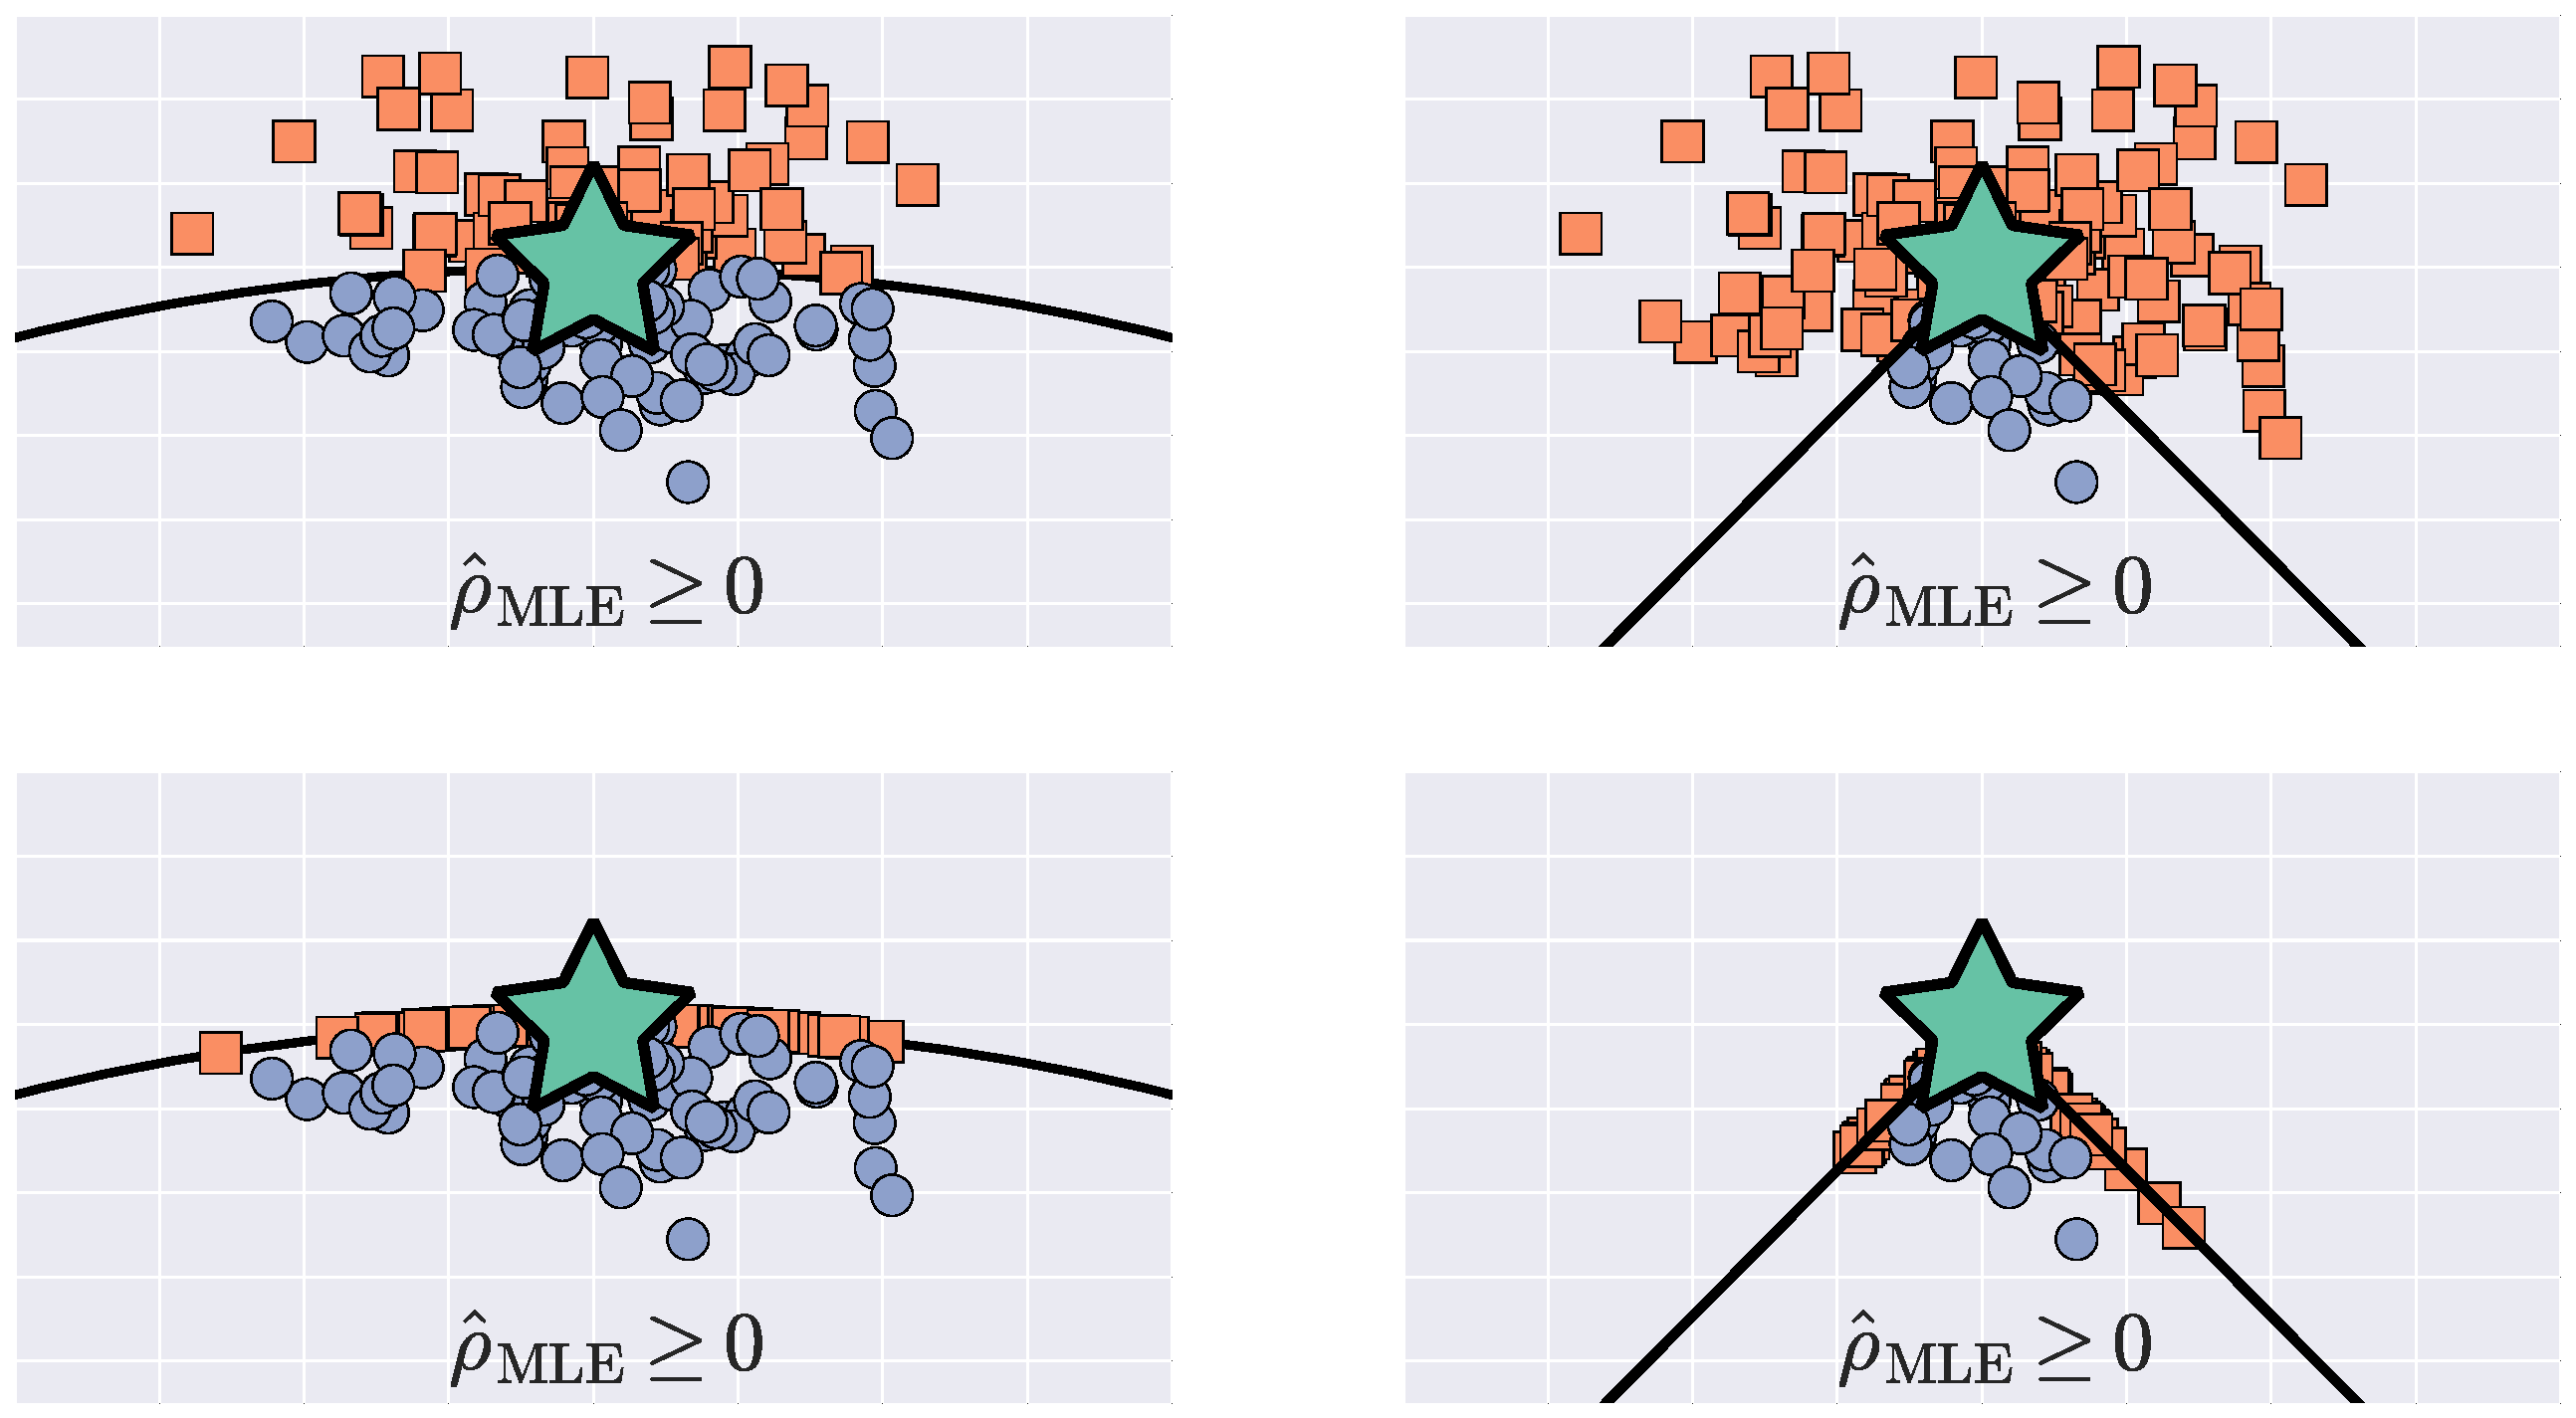
\includegraphics[width=\columnwidth]{Images/Figure_1.pdf}
 \caption{Impact of the boundary on maximum likelihood tomography. \textbf{Top}: Two views through the qutrit state space. Without the positivity constraint, some estimates (orange squares) are not positive semidefinite, and do not represent valid estimates of a quantum state. The distribution of $\rhoMLE$ (blue circles) is generally non-normal, and depends on the true state $\rho_{0}$ (star).
\textbf{Bottom}:  Comparison of the classical theory (Wilks Theorem) prediction for the loglikelihood ratio $\expect{\lambda}$ to numerical data for states $\rho_{0}$ with ranks $r=1,\ldots ,10$.  The Wilks Theorem fails badly for low-rank states; our main result (Equation \ref{eq:ourLLRS}) fixes this problem (see Figure \ref{fig:modelcomp-iso}).}
\label{fig:boundaries}
\end{figure}

\section{Quantum State Tomography and Model Selection}
As mentioned above, the Born rule is the bridge which relates state tomography to statistical inference. A basic state tomography protocol proceeds as follows. Suppose we have access to $N$ copies of an unknown state $\rho_{0}$. For each copy, we measure some POVM, and record the outcome obtained. Repeating the measurement of the POVM on all $N$ copies, we will generate data in the form of a record of the number of times we saw different outcomes: $\mathrm{Data} = \{(n_{j}, E_{j})\}$, with $n_{j}$ as the number of times outcome $E_{j}$ was observed, and $\sum_{j}n_{j} = N$. The task of state tomography is to process this data, and provide an estimate of $\rho_{0}$. As we are concerned with computing the likelihood of a model $\M$, which is given by the likelihood of the most likely state within it, we need some way of finding the maximum likelihood over all the parameters of $\M$. A straightforward (though often computationally intensive) way is to compute the maximum likelihood estimate $\rhoMLE$ itself, thereby allowing us to calculate the likelihood of $\M$ as $\mathcal{L}(\rhoMLE)$. (Of course, it may be possible to calculate $\mathcal{L}(\rhoMLE)$ \emph{without} computing $\rhoMLE$ itself.) Below, we briefly describe how $\rhoMLE$ is calculated.

Given the data, $\rhoMLE$ is the state which which maximizes the probability of the observed data. Assuming the POVM elements are measured independently, the likelihood $\mathcal{L}(\rho)$ is
\begin{equation}
\mathcal{L}(\rho) = \prod_{j}\mathrm{Tr}(\rho E_{j})^{n_{j}}.
\end{equation}
For some model $\M$, $\rhoMLE$ is the solution to the optimization problem
\begin{equation}
\rhoMLE = \underset{\rho \in \M}{\text{argmax}}~\mathcal{L}(\rho).
\end{equation}
Typically, $\M$ is taken to be the set of all density matrices over some Hilbert space $\cH$, which is usually chosen by fiat. $\M$ is convex, which allows for the use of efficient algorithms for finding $\rhoMLE$ \cite{Boyd}. For our model selection problem, we will be considering a nested family of different Hilbert spaces, indexed by their dimension $d$: $\cH_{1}  \subset \cdots \cH_{d} \subset \cH_{d+1} \subset \cdots$.

Given a Hilbert space $\cH_{d}$, we define the model $\mathcal{M}_{d}$ as
\begin{equation}
\mathcal{M}_{d} = \{\rho~|~\rho \in \mathcal{B}(\mathcal{H}_{d}),~\mathrm{Tr}(\rho) =1,~\rho \geq 0\},
\end{equation}
where $\mathcal{B}(\cH_{d})$ is the space of bounded operators on $\cH_{d}$. Model selection for $d$ involves evaluating whether $\M_{d + 1}$ is a better model than $\M_{d}$. To answer that question, we need a null theory for $\lambda$ (i.e, its behavior when $\rho_{0} \in \M_{d},\M_{d + 1}$).

In classical statistics, the null theory for $\lambda$ (the Wilks Theorem) relies on LAN.  If LAN holds, the likelihood function near $\rhoMLE$ is given by \footnote{Here, we are using the \emph{vector notation}, so that each state $\rho \rightarrow \mathrm{vec}(\rho) = |\rho)$, which returns a column vector with $d^{2}$ entries. In turn, $\mathcal{I}$ and $\mathcal{I}^{-1}$ are $d^{2}\times d^{2}$ operators on the vector space.}
\begin{equation}
\mathcal{L}(\rho) \propto \text{Exp}\left[-(\rho - \rhoMLE|\mathcal{I}^{-1}|\rho - \rhoMLE)/2\right],
\end{equation}
and the distribution of $\rhoMLE$ is
\begin{equation}
\mathrm{Pr}(\rhoMLE) \propto \text{Exp}\left[-(\rho_{0} - \rhoMLE|\mathcal{I}|\rho_{0} - \rhoMLE)/2\right],
\end{equation}
\todo[inline]{Is the inverse in the right place?}
where $\mathcal{I}$ is the Fisher information. In classical statistics, it is common to assume that the models either do not have boundaries (such as vector spaces), or that the true parameter values $\rho_{0}$ lie sufficiently far from the boundary that its existence is not a concern. Either assumption allows the statistician to do a co\"{o}rdinate transformation to bring the Fisher information into an isotropic form, which greatly simplifies the analysis of the problem. In state tomography, $\mathcal{I}$ is generally anisotropic. \todo[inline]{See Figure ??} However, performing a co\"{o}rdinate transformation in state space then distorts its geometry; in particular, the positivity constraint $\rho \geq 0$ becomes difficult to compute analytically. Thus, in this paper, we make the simplifying assumption that $\mathcal{I}$ is proportional to the Hilbert-Schmidt metric ($\mathcal{I} \propto \mathbb{I}$).  

When $\rho_{0}$ is full-rank in $\M_{d}$, LAN will hold. In this case, the null theory for $\lambda$ is given by the Wilks Theorem: $\lambda(\M_{d}, \M_{d + 1}) \sim \chi^{2}_{2d + 1}$. However if $\rho_{0}$ is rank-deficient, then the boundary looms, and $\mathrm{Pr}(\rhoMLE)$ is not Gaussian. This distortion occurs, even in the asymptotic limit,  precisely when $\rho_{0}$ is rank-deficient within $\cH_{d}$. (That is, when $\rho_{0}$ is on the boundary of $\cH_{d}$. See Figure \ref{fig:boundaries}.) If $\mathrm{Pr}(\rhoMLE)$ is not Gaussian, LAN does not hold, and the Wilks Theorem does not apply! Crucially, \emph{even if $\rho_{0}$ is full-rank in $\M_{d}$, it will be rank-deficient in $\M_{d+1}$}. Thus, if we want to use model selection to choose $d$ in state tomography, we must understand the null behavior of $\lambda$ -- i.e., derive a replacement Wilks Theorem -- for rank-deficient $\rho_{0}$. Because $\mathrm{Pr}(\rhoMLE)$ is complicated, depending strongly on the local geometry of the state space around $\rho_{0}$, we will not attempt to compute $\mathrm{Pr}(\lambda)$ directly. Instead, we approximate $\langle \lambda \rangle$. Deriving this approximation under the assumption $\mathcal{I} \propto \Id$ is the bulk of the remaining content of this paper; to jump straight to the result, see Equation \eqref{eq:ourLLRS}.

\missingfigure{Picture of $\rhohat$, $\rhoMLE$, etc. w/ anisotropic Fisher information}

\section{Deriving a Replacement for the Wilks Theorem}

In this section, we show how to derive a replacement for the Wilks Theorem which is valid for rank-deficient $\rho_{0}$. 
To do so, we start by making assumptions about likelihood $\mathcal{L}(\rho)$; namely, that, over the set of bounded, trace-one operators in $\mathcal{B}(\mathcal{H}_{d})$, LAN holds. We will focus on the special and simple case where $\Fi$ at $\rho_{0}$ is  proportional to the Hilbert-Schmidt metric, so the likelihood function (and the distribution of the \emph{unconstrained} MLEs $\rhohat$) is given by 
\todo[inline]{We've used MLE = maximum likelihood estimation. Is it confusing to do MLE = maximum likelihood estimate?}
\begin{align}
\label{eq:likelihood}
\cL(\rho) & \propto e^{-\mathrm{Tr}[(\rho - \rhohat)^{2}]/2\epsilon^{2}}\\
\mathrm{Pr}(\rhohat) &\propto e^{-\mathrm{Tr}[(\rho_{0} - \rhohat)^{2}]/2\epsilon^{2}}
\end{align}
for some $\epsilon$ that scales as $1 / \sqrt{N_{\mathrm{samples}}}$.  The isotropic assumption greatly simplifies our study of the problem, and permits the derivation of analytic results which capture realistic tomographic scenarios surprisingly well \cite{Smolin2012}. 
Because it is unconstrained, $\rhohat$ is often not positive semidefinite (see Figure \ref{fig:boundaries}). For each $\rhohat$, the MLE in $\M_{d}$, $\hat{\rho}_{\mathrm{MLE},d}$ is the solution to the following optimization problem:
\begin{equation}
\label{eq:mleopt}
\hat{\rho}_{\mathrm{MLE}, d} = \underset{\rho \in \M_{d}}{\mathrm{argmin}}~\mathrm{Tr}[(\rhohat - \rho)^{2}].
\end{equation}

In turn, $\lambda(\M_{d}, \M_{d+1})$ is given by
\begin{equation}
\label{eq:llrs}
\lambda(\M_{d}, \M_{d+1}) = \frac{\mathrm{Tr}[(\hat{\rho}_{\mathrm{MLE}, d}  - \rhohat)^{2}] - \mathrm{Tr}[(\hat{\rho}_{\mathrm{MLE}, d+1} - \rhohat)^{2}]}{\epsilon^{2}}.
\end{equation}

Our derivation of $\langle \lambda \rangle$ involves three main steps:
\begin{itemize}
\item Reduce calculating $\langle \lambda(\M_{d}, \M_{d+1})\rangle$ to that of computing mean-squared errors $\langle \mathrm{Tr}[(\hat{\rho}_{\mathrm{MLE},d} - \rho_{0})^{2}]\rangle$.
\item Separate out degrees of freedom in $\rhohat$ which are unaffected by the positivity constraint, and those which are.
\item For the degrees of freedom of $\rhohat$ which are affected by the positivity constraint (which will turn out to be \emph{spectral} in nature), derive an analytic approximation to the optimization problem given in Equation \eqref{eq:mleopt}.
\end{itemize}

\subsection{Relating $\langle \lambda \rangle$ to Mean-Squared Error}

To simplify our derivation, we first show how we may reduce the problem of computing the expected value of $\lambda$ given in Equation \eqref{eq:llrs} to that of computing the mean-squared error between $\hat{\rho}_{\mathrm{MLE},d}$ and $\rho_{0}$. We start by relating $\lambda(\M_{d},\M_{d+1})$ to $\lambda(\rho_{0}, \M_{d})$ and $\lambda(\rho_{0}, \M_{d+1})$ using the identity
\begin{equation}
\lambda(\mathcal{M}_{d}, \mathcal{M}_{d + 1}) = \lambda(\rho_{0}, \mathcal{M}_{d+1}) - \lambda(\rho_{0}, \mathcal{M}_{d}),
\end{equation}
where
\begin{align}
\nonumber\lambda(\rho_{0}, \mathcal{M}_{d}) &= -2 \log \left(\frac{\mathcal{L}(\rho_{0})}{\underset{\rho \in \mathcal{M}_{d}}{\max}
\mathcal{L}(\rho)}\right)\\
& = (\mathrm{Tr}[(\rho_{0} - \hat{\rho})^{2}]- \mathrm{Tr}[(\rhoMLE - \hat{\rho})^{2}])/\epsilon^{2}.
\end{align}
This identity may be interpreted as saying that when evaluating the plausibility of two models, we may compare each to any \emph{reference model}. Here, we take that reference model to be the $\rho_{0}$ itself.

Now, we derive an equivalent expression for $\lambda(\rho_{0}, \M_{d})$. To do so, we show that replacing the local state space with a \emph{tangent cone} at $\rho_{0}$, denoted $C(\rho_{0})$ allows us to ???

\todo[inline]{What does it allow us to do, succinctly?}

\todo[inline]{Check these definitions}
\textbf{Definition}: Given a state $\rho_{0}\in \M_{d}$, the tangent cone at $\rho_{0}$, denoted $C(\rho_{0})$ is given by the closure of the set of rays emanating from $\rho_{0}$ to any $\sigma \in \M_{d}$.

For example, if $\rho_{0}$ is a pure state in $\M_{2}$, then $C(\rho_{0})$ is the two-dimensional plane which touches the surface of the Bloch sphere at $\rho_{0}$. If $\rho_{0}$ is a mixed state in $\M_{2}$, $C(\rho_{0})$ is $\mathbb{R}^{3}$.

Notice that $\M_{d} \subset C$, by construction. With the tangent cone defined, we now define the maximum likelihood estimate within it.

\textbf{Definition} Given $\hat{\rho}$, and the tangent cone $C(\rho_{0})$, define $\hat{\rho}_{\mathrm{MLE}, C}$ as the solution to the following optimization problem:
\begin{equation}
\hat{\rho}_{\mathrm{MLE}, C} = \underset{M \in C}{\text{argmin}}~\mathrm{Tr}[(M - \rhohat)^{2}]
\end{equation}
Note that $\hat{\rho}_{\mathrm{MLE}, C}$ \emph{need not be positive semi-definite}!

\textbf{Definition} Define the loglikelihood ratio statistic comparing $\rho_{0}$ to the model $C(\rho_{0})$ as 
\begin{align}
\nonumber\lambda(\rho_{0}, C) &\equiv -2 \log \left(\frac{\mathcal{L}(\rho_{0})}{\mathcal{L}(\hat{\rho}_{\mathrm{MLE}, C})}\right)\\
\label{eq:tangentLLRS}
& = (\mathrm{Tr}[(\rho_{0} - \rhohat^{2})] - \mathrm{Tr}[(\hat{\rho}_{\mathrm{MLE}, C} - \rhohat)^{2}])/\epsilon^{2}
\end{align}

\missingfigure{Picture of Pythagorean Theorem}

It turns out $\lambda(\rho_{0}, C)$ has a particularly pleasing form.

\textbf{Theorem} $\lambda(\rho_{0}, C) = \mathrm{Tr}[(\rho_{0} - \hat{\rho}_{\mathrm{MLE}, C})^{2}]$.

\textbf{Proof}

\emph{Case 1}: Assume $\rhohat \not \in C$. Because $\hat{\rho}_{\mathrm{MLE}, C}$ is the closest point to $\rhohat$ in $C$, and because $C$ contains $\rho_{0}$, the lines joining $\rho_{0}$ to $\hat{\rho}_{\mathrm{MLE}, C}$, and $\hat{\rho}_{\mathrm{MLE}, C}$ to $\rhohat$, are at right angles to one another. (See Figure ??) Applying the Pythagorean theorem, we have
\begin{equation}
\label{eq:pythag}
\mathrm{Tr}[(\rho_{0} - \rhohat)^{2}] = \mathrm{Tr}[(\rho_{0} - \hat{\rho}_{\mathrm{MLE}, C})^{2}] + \mathrm{Tr}[(\rhohat - \hat{\rho}_{\mathrm{MLE}, C})^{2}]
\end{equation}
Dividing Equation \eqref{eq:pythag} by $\epsilon^{2}$, and combining with Equation \eqref{eq:tangentLLRS}, yields the theorem statement.

\emph{Case 2}: Assume $\rhohat \in C$. Then, $\hat{\rho}_{\mathrm{MLE}, C} = \rhohat$, and Equation \eqref{eq:tangentLLRS} simplifies to the theorem statement.
~\\~\\
Finally, it turns out that as $\epsilon \rightarrow 0$, the values of $\lambda(\rho_{0}, \M_{d})$ and $\lambda(\rho_{0}, C)$ coincide.

\textbf{Theorem} $\lim_{\epsilon \rightarrow 0} [\lambda(\rho_{0}, \M_{d}) - \lambda(\rho_{0}, C)] = 0$
\todo[inline]{Or is it in expectation? Or what?}
\textbf{Proof} We consider three cases:

\emph{Case 1}: $\rhohat \in \M_{d}$. In this case, $\rhoMLE = \hat{\rho}_{\mathrm{MLE}, C} = \rhohat$, so $\lambda(\rho_{0}, \M_{d}) = \lambda(\rho_{0}, C)$, and the limit trivially holds.

\emph{Case 2}: $\rhohat \not \in \M_{d}$, but $\rhohat \in C$. In this case, $\hat{\rho}_{\mathrm{MLE}, C} = \rhohat$, so $\epsilon^{2}\lambda(\rho_{0}, C) = \mathrm{Tr}[(\rho_{0}-\hat{\rho}_{\mathrm{MLE}, C})^{2}]$, and $\epsilon^{2}\lambda(\rho_{0}, \M_{d}) = \mathrm{Tr}[(\rho_{0} - \hat{\rho}_{\mathrm{MLE}, C})^{2}] - \mathrm{Tr}[(\rhoMLE - \hat{\rho}_{\mathrm{MLE}, C})^{2}]$. So we have
\[\lambda(\rho_{0}, \M_{d}) - \lambda(\rho_{0}, C) = -\frac{1}{\epsilon^{2}}\mathrm{Tr}[(\rhoMLE - \hat{\rho}_{\mathrm{MLE}, C})^{2}]\] 
\todo[inline]{And???}
\emph{Case 3}: $\rhohat \not \in \M_{d}, C$. In this case, $\epsilon^{2}\lambda(\rho_{0}, C) = \mathrm{Tr}[(\rho_{0} - \rhohat^{2})] - \mathrm{Tr}[(\hat{\rho}_{\mathrm{MLE}, C} - \rhohat)^{2}]$ and $\epsilon^{2}\lambda(\rho_{0},\M_{d}) = \mathrm{Tr}[(\rho_{0} - \hat{\rho})^{2}]- \mathrm{Tr}[(\rhoMLE - \hat{\rho})^{2}]$, so

\[\lambda(\rho_{0}, \M_{d}) - \lambda(\rho_{0}, C) = \frac{1}{\epsilon^{2}}\left[\mathrm{Tr}[(\hat{\rho}_{\mathrm{MLE}, C} - \rhohat)^{2}] -  \mathrm{Tr}[(\rhoMLE - \hat{\rho})^{2}]\right]\]

Consider a triangle whose vertices are located at $\rhoMLE, \rhohat$, and $\hat{\rho}_{\mathrm{MLE}, C}$. Defining $\theta$ as the angle between $\rhoMLE - \rhohat$ and $\hat{\rho}_{\mathrm{MLE}, C} - \rhohat$, $A$ as $\sqrt{\mathrm{Tr}[(\rhoMLE - \hat{\rho})^{2}]}$, $B$ as $\sqrt{\mathrm{Tr}[(\rhoMLE - \hat{\rho}_{\mathrm{MLE}, C})^{2}]}$, and $C$ as $\sqrt{\mathrm{Tr}[(\hat{\rho}_{\mathrm{MLE}, C} - \rhohat)^{2}]}$ (see Figure ??), we then have
\[\lambda(\rho_{0}, \M_{d}) - \lambda(\rho_{0}, C) = \frac{1}{\epsilon^{2}}\left[C^{2} - A^{2}\right]\]

An application of the law of cosines yields
\[C^{2} = A^{2} + B^{2} - 2AB\cos\theta\]
which implies
\[\lambda(\rho_{0}, \M_{d}) - \lambda(\rho_{0}, C) = \frac{1}{\epsilon^{2}}\left[B^{2} - 2AB\cos\theta\right]\]
which, in terms of the original variables, means
\begin{align}
\nonumber \epsilon^{2}(\lambda(\rho_{0}, \M_{d}) - \lambda(\rho_{0}, C)) = \mathrm{Tr}[(\rhoMLE - \hat{\rho}_{\mathrm{MLE}, C})^{2}]\\
-2\sqrt{\mathrm{Tr}[(\rhoMLE - \hat{\rho})^{2}]\mathrm{Tr}[(\rhoMLE - \hat{\rho}_{\mathrm{MLE}, C})^{2}]}\cos\theta
\end{align}
\missingfigure{Picture for Case 3}

\todo[inline]{And??}

\todo[inline]{Need to show that $B^{2}$ either goes as $\epsilon^{3}$ or higher, or is $\mathcal{O}(\epsilon^{2})$}

To summarize, through these identities and approximations, we have reduced the problem of computing $\lambda(\M_{d}, \M_{d+1})$ to that of computing the (scaled) mean-squared error $\mathrm{Tr}[(\rhoMLE - \rho_{0})^{2}]/\epsilon^{2}$ for each $\hat{\rho}_{\mathrm{MLE},d}$ in both $\M_{d}$ and $\M_{d+1}$ by replacing the local state space with a tangent cone.
Now, we must determine an approximate form for $\langle\mathrm{Tr}[(\rhoMLE - \rho_{0})^{2}]\rangle/\epsilon^{2}$.

\subsection{Separating out Degrees of Freedom in $\rhohat$}

We begin by observing that $\lambda(\rho_{0}, \M_{d})$ can be written as a sum over matrix elements,
\begin{align}
\label{eq:llrserrors}
\nonumber \lambda &=\epsilon^{-2}\mathrm{Tr}[(\rhoMLE - \rho_{0})^{2}] = \epsilon^{-2}\sum_{jk}|(\rhoMLE- \rho_{0} )_{jk}|^{2}\\
&= \sum_{jk}\lambda_{jk}~~~~\text{where}~~~~\lambda_{jk} = \epsilon^{-2}|(\rhoMLE - \rho_{0} )_{jk} |^{2},
\end{align}
and therefore $\langle \lambda \rangle = \sum_{jk}\langle\lambda_{jk}\rangle$.  Each term $\langle \lambda_{jk}\rangle$ quantifies the average mean-squared error of a single matrix element of $\rhoMLE$, and while the Wilks Theorem predicts $\expect{\lambda_{jk}}=1$ for all $j,k$, numerical simulations (see Figure \ref{fig:L}) show that this only holds true for \emph{some} matrix elements.  A few contribute more than 1 unit (on average) while many others contribute much less, meaning that the Wilks Theorem predicts too high a value for the total $\expect{\lambda}$.  (See bottom of Figure \ref{fig:boundaries}.) Thus motivated, we divide the parameters of $\rhohat$ into two parts (see Figure \ref{fig:L}),
\begin{enumerate}[noitemsep]
\item The ``kite'' comprises all diagonal elements \emph{and} all elements on the kernel (null space) of $\rho_0$,
\item The ``L'' comprises all off-diagonal elements on the support of $\rho_0$ \emph{and} between the support and the kernel,
\end{enumerate}
and observe that $\langle\lambda\rangle = \expect{\lambda_{\mathrm{L}}} + \expect{\lambda_{\mathrm{kite}}}$.  The rationale for this division is simple:  small fluctuations on the ``L'' do not change the zero eigenvalues of $\hat\rho$ to 1$^{\mathrm{st}}$ order, whereas those on the ``kite'' do. In what follows, we study how imposing the positivity constraint $\rhoMLE \geq 0$ affects the behavior of the matrix elements in each part.

\begin{figure}[h]
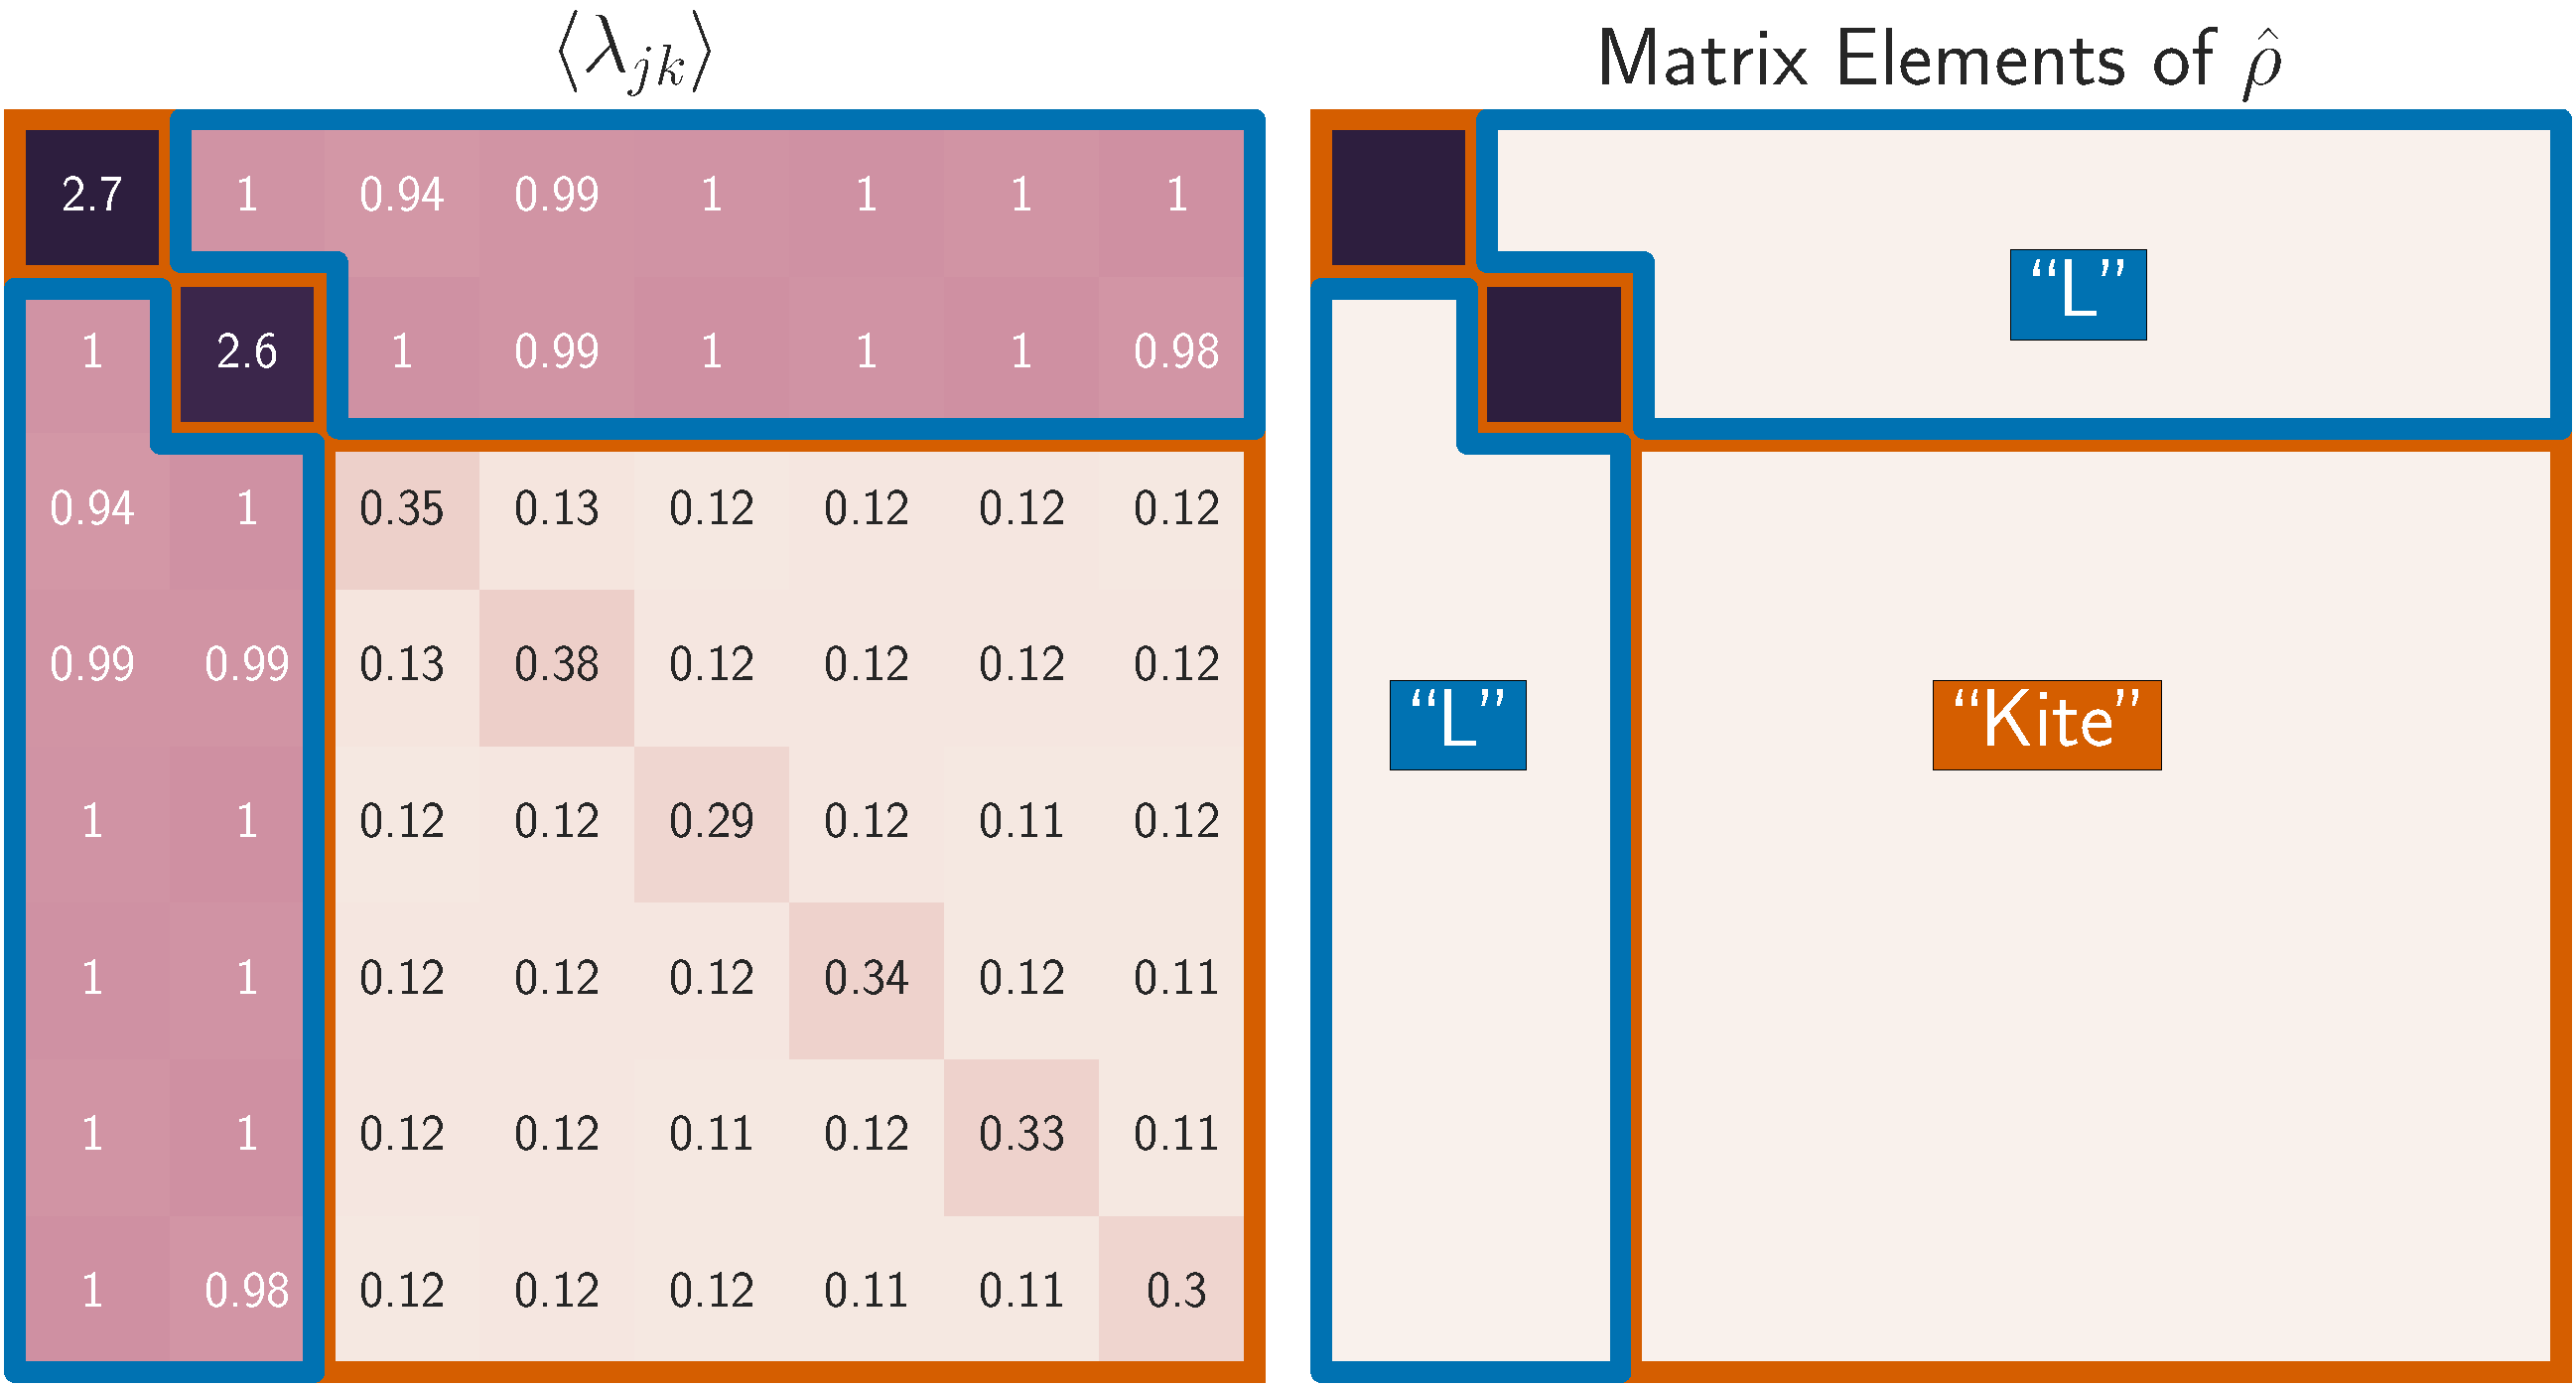
\includegraphics[width=\columnwidth]{Images/Figure_2.pdf}
 \caption{When a rank-2 state is reconstructed in $d=8$ dimensions, the total loglikelihood ratio $\lambda(\rho_0,\mathcal{M}_8)$ is the sum of terms $\lambda_{jk}$ from errors in each matrix element $(\rhoMLE)_{jk}$.  \textbf{Left}:  Numerics show a clear division; some matrix elements have $\expect{\lambda_{jk}}\sim1$ as predicted by the Wilks Theorem, while others are either more or less. \textbf{Right}:  The numerical results motivate dividing the elements of $\rhohat$ into two parts: the ``kite'' and the ``L''.}
\label{fig:L}
\end{figure}

In doing so, it is helpful to think about the error of the unconstrained estimate $\delta \equiv \hat\rho- \rho_{0}$, a normally-distributed \emph{traceless} matrix.  To simplify the analysis, we explicitly drop the $\Tr(\rho)=1$ constraint and let $\delta$ be $\mathcal{N}(0,\epsilon^2\Id)$ distributed over the $d^2$-dimensional space of Hermitian matrices (a good approximation when $d\gg2$) \footnote{That is, we let $\mathrm{Tr}(\delta)$ fluctuate as well.}, which makes $\delta$ proportional to an element of the Gaussian Unitary Ensemble (GUE) \cite{Fyodorov2005}.

\subsubsection{Computing $\langle \lambda_\mathrm{L}\rangle$}

To first order in $\epsilon$, elements of $\delta$ in the ``L'' do not affect positivity, so they are unconstrained by the boundary, and behave exactly as expected from classical theory. The $\delta_{jk}$ in the ``L'' may be seen as errors which arise due to small unitary perturbations of $\rho_{0}$. Writing $\rhohat = U^{\dagger}\rho_{0}U$, where $U=e^{i\epsilon H}$, we have
\[\rhohat \approx \rho_{0} + i\epsilon [\rho_{0},H]+\mathcal{O}(\epsilon^{2}).\]
Then, $\delta \approx i\epsilon [\rho_{0},H]$.
If $j = k$, then $\delta_{jj} = 0$. Thus, small unitaries cannot create errors in the diagonal matrix elements, at $\mathcal{O}(\epsilon)$. If $j \neq k$, then $\delta_{jk} \neq 0$, in general. (Small unitaries \emph{can} introduce errors on off-diagonal elements.)

However, if either $j$ or $k$ (or both) lie within the \emph{kernel} of $\rho_{0}$ (i.e., $\langle k | \rho_{0}| k \rangle$ or $\langle j|\rho_{0}|j\rangle$ is 0), then the corresponding $\delta_{jk}$ are zero. The only off-diagonal elements where small unitaries can introduce errors are those which are coherent between the kernel of $\rho_{0}$ and its support. These off-diagonal elements are precisely the ``L", and are  the set $\{\delta_{jk}~|~\langle j | \rho_{0}|j\rangle \neq 0, j\neq k, ~ 0 \leq j,k \leq d - 1\}$. Each $\delta_{jk}$ in the ``L'' is a $\mathcal{N}(0, \epsilon^{2})$ random variable, and crucially, is identical to the error $(\rhoMLE - \rho_{0})_{jk}$. This is because these $\delta_{jk}$ are \emph{unaffected by the boundary}, so when we impose the positivity constraint (i.e., compute $\rhoMLE$), their values remain the same. Therefore, $\langle \lambda_{jk}\rangle = \langle \delta_{jk}^{2}\rangle /\epsilon^{2} = 1$. As there are $2rd - r(r+1)$ of them, $\expect{\lambda_{\mathrm{L}}} = 2rd - r(r+1)$.

\subsubsection{Setting the Stage to Compute $\langle \lambda_\mathrm{kite}\rangle$}

We next need a procedure to compute $\rhoMLE$ given $\rhohat$ -- i.e., to solve the optimization problem in Eq. \eqref{eq:mleopt}.  Fortunately, an algorithm for doing so was presented in Ref. \cite{Smolin2012}:
\begin{enumerate}[noitemsep]
\item Subtract $q\Id$ from the unconstrained $\hat\rho$, for a particular real scalar $q$,
\item ``Truncate'' $\hat\rho-q\Id$, by replacing each of its negative eigenvalues with zero.
\end{enumerate}
Here, $q$ is defined implicitly such that $\Tr\left[ \mathrm{Trunc}(\hat\rho-q\Id)\right] = 1$.

Although this was intended as a (very fast) numerical algorithm, we will manipulate it (by a series of approximations) to derive a closed-form expression for the average $\expect{\lambda}$.  

Computing $\expect{\lambda_{\mathrm{kite}}}$ is a bit harder, because the boundary \emph{does} constrain its elements.  Here, we turn to the truncation algorithm given above for finding $\rhoMLE$, which is most naturally performed in the eigenbasis of $\hat\rho$.  Exact diagonalization of $\hat\rho$ is not feasible analytically, but only the \emph{small} eigenvalues of $\hat\rho$ are critical in truncation.  As long as all the nonzero eigenvalues of $\rho_0$ are much larger than $\epsilon$, the eigenbasis of $\hat\rho$ is accurately approximated by: (1) 
the eigenvectors of $\rho_0$ on its support; and (2) the eigenvectors of $\delta_{\mathrm{ker}} = \Pi_{\mathrm{ker}}\delta\Pi_{\mathrm{ker}}$, where $\Pi_{\mathrm{ker}}
$ is the projector onto the kernel of $\rho_0$.

Changing to this basis diagonalizes the ``kite'' portion of $\delta$, and leaves all elements of the ``L'' unchanged (at $\mathcal{O}(\epsilon)$).  The diagonal elements of $\hat\rho$ now fall into two categories:
\begin{enumerate}[noitemsep]
\item $r$ elements corresponding to the eigenvalues of $\rho_0$, which are given by $p_{j} = \rho_{jj} + \delta_{jj}$ where  $\rho_{jj}$ is the $j^{\mathrm{th}}$ eigenvalue of $\rho_{0}$, and $\delta_{jj} \sim \mathcal{N}(0,\epsilon^2)$.
\item $N \equiv d-r$ elements that are eigenvalues of $\delta_{\mathrm{ker}}$, which we denote by $\bvec{\kappa} = \{\kappa_j:~j = 1\ldots 
N\}$,
\end{enumerate}
and $\lambda_{\mathrm{kite}}$ is
\begin{equation}
\label{eq:llrs_kite}
\epsilon^{2}\lambda_{\mathrm{kite}} = \sum_{j=1}^{r}[\rho_{jj}- (p_j-q)^{+}]^2 + \sum_{j=1}^{N}\left[(\kappa_j-q)^+\right]^2,
\end{equation}
where $(x)^{+} = \max(x, 0)$. $q$ is implicitly defined such that $f(q) \equiv \Tr\left[\mathrm{Trunc}(\hat\rho - q \Id)\right]$ satisfies $f(q) = 1$. In terms of the eigenvalues of $\rhohat$, this means $q$ is the solution to
\begin{equation}
\label{eq:q_eqn}
 \sum_{j=1}^{r}(p_j - q)^{+} + \sum_{j=1}^{N}{(\kappa_j-q)^+} = 1
\end{equation}

To solve Equation \eqref{eq:q_eqn}, and derive an approximation for \eqref{eq:llrs_kite}, we need to understand the behavior of the eigenvalues of $\delta_{\mathrm{ker}}$. It is to this problem we now turn.

\subsubsection{Approximating the Eigenvalues of a GUE($N$) Matrix}
We first observe that while the $\kappa_j$ are random variables, they are not normally distributed.  Instead, because $\delta_{\mathrm{ker}}$ is proportional to a $\mathrm{GUE}(N)$ matrix, for $N\gg1$, the distribution of any eigenvalue $\kappa_{j}$
converges to a Wigner semicircle distribution \cite{Wigner1958} given by $\mathrm{Pr}(\kappa) = \frac{2}{\pi R^{2}}\sqrt{R^{2}-\kappa^{2}}$ for $|\kappa| \leq R$, with $R = 2\epsilon\sqrt{N}$.  The eigenvalues are not independent; they tend to avoid collisions (``level avoidance'' \cite{Tao2013}), 
and typically form a surprisingly regular array over the support of the Wigner semicircle.  Since our goal is to compute $\expect{\lambda_{\mathrm{kite}}}$, we can capitalize on this behavior by replacing each random sample of $\bvec{\kappa}$ with a 
\emph{typical sample} $\bar{\bvec{\kappa}}$ given by its order statistics.  These are the average values of the \emph{sorted} 
$\bvec{\kappa}$, so $\overline{\kappa}_j$ is the average value of the $j^{\mathrm{th}}$ largest value of $\bvec{\kappa}$.  Large random samples 
are usually well approximated (for many purposes) by their order statistics even when the elements of the sample are 
independent, and level avoidance makes the approximation even better. 

\begin{figure}[h!]
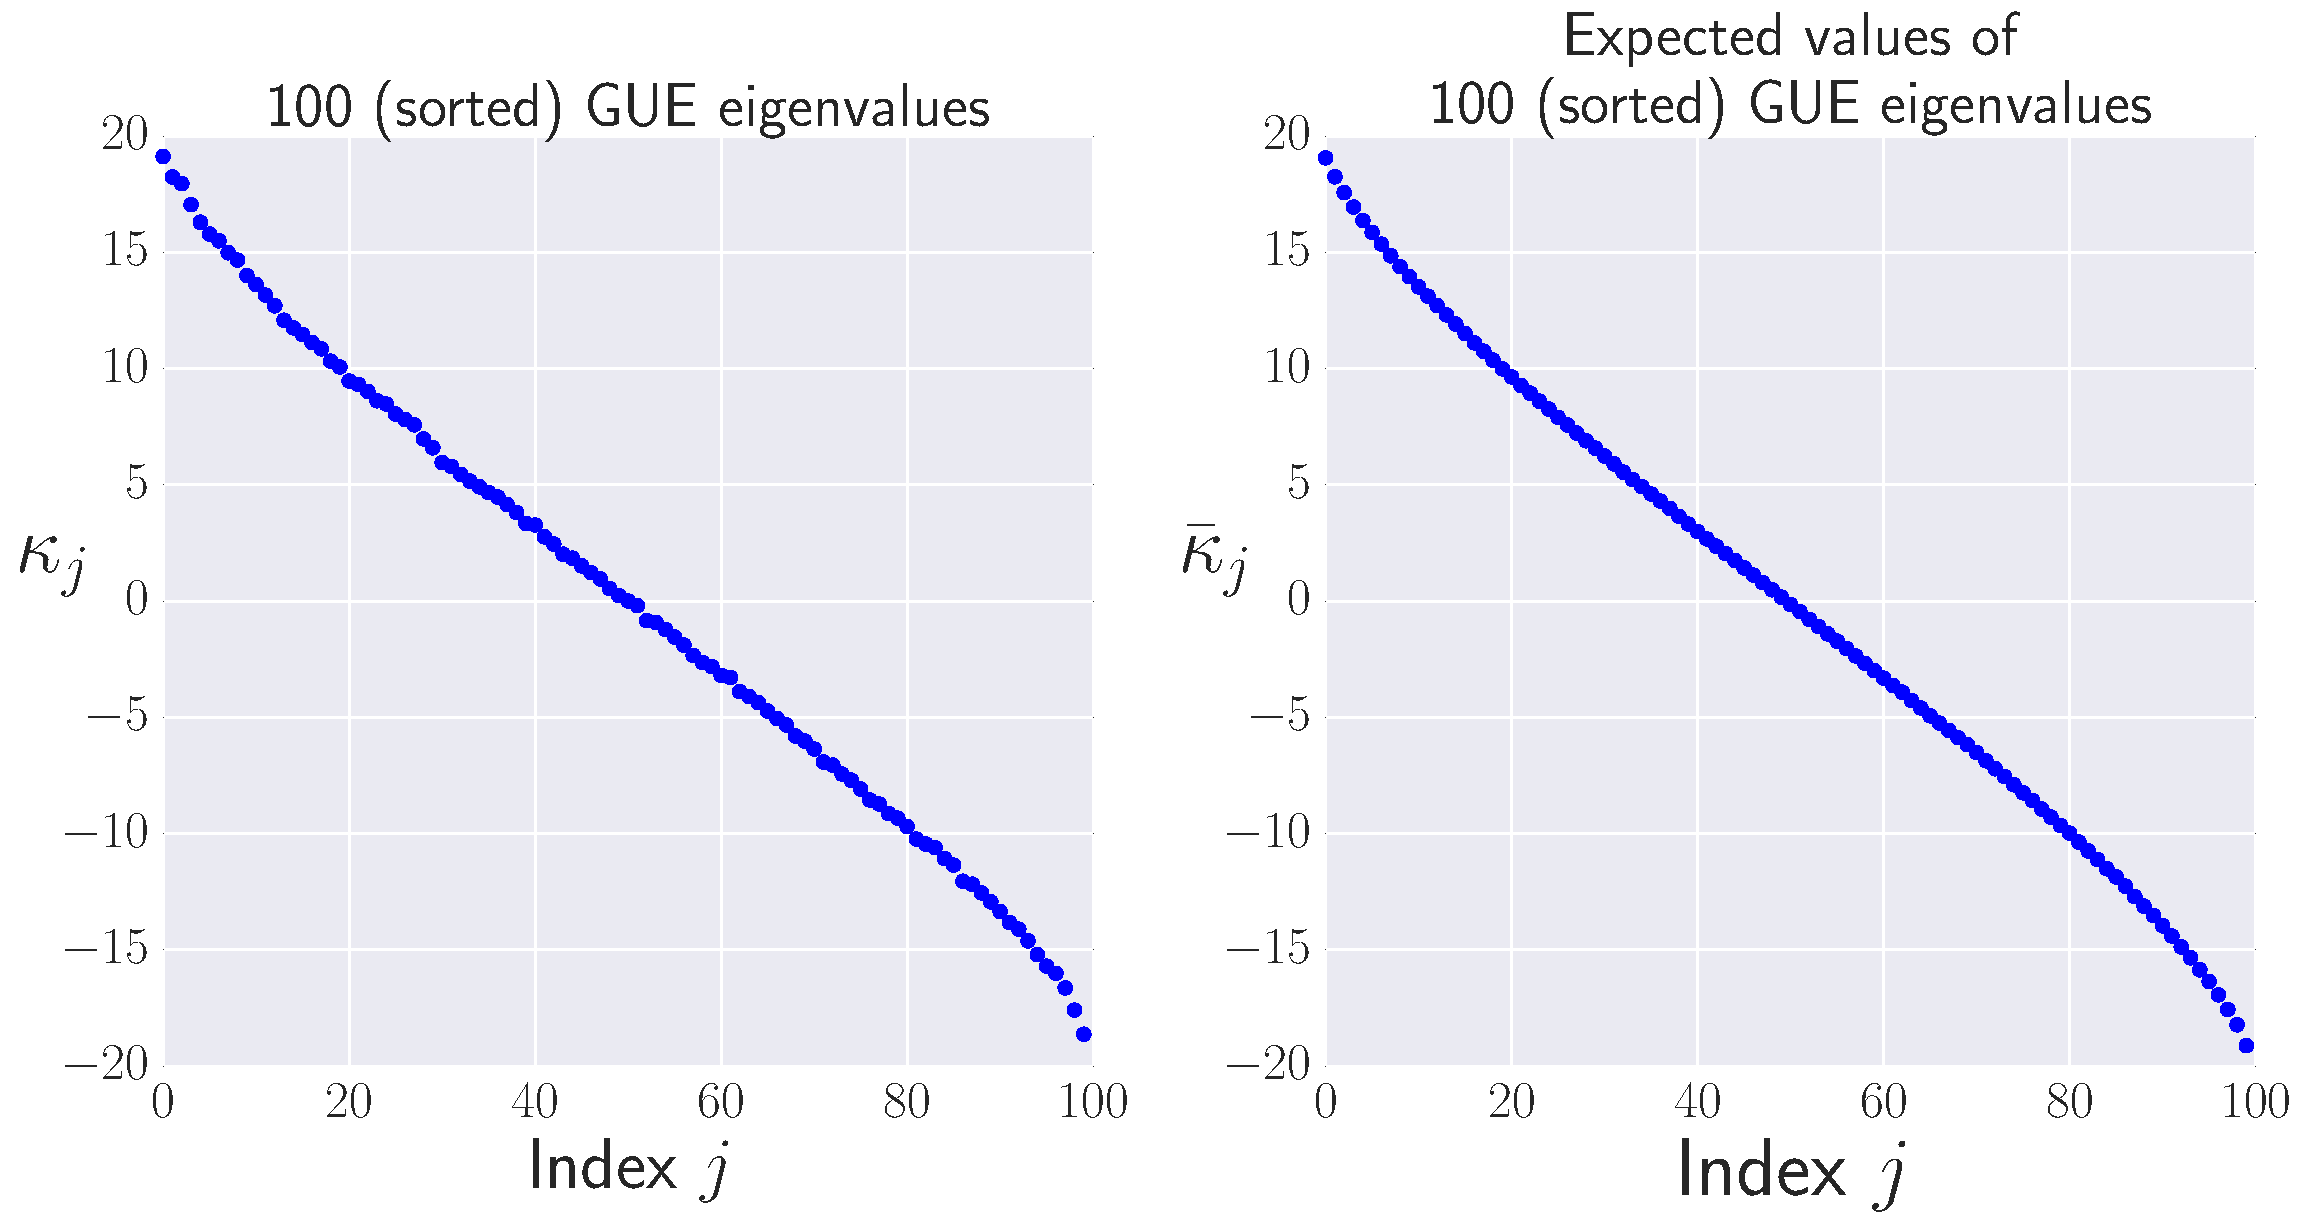
\includegraphics[width=\columnwidth]{Images/Figure_3.pdf}
\caption{Typical samples of GUE($N$) eigenvalues are accurately approximated by order statistics of the distribution (average values of a sorted sample).  \textbf{Left}:  The sorted eigenvalues (i.e., order statistics $\kappa_{j}$) of one randomly chosen GUE(100) matrix.  \textbf{Right}:  Approximate expected values of the order statistics, $\bar{\kappa}_{j}$, of the GUE(100) distribution, computed as the average of the sorted eigenvalues of 100 randomly chosen GUE(100) matrices.}
\label{fig:orderstatistics1}
\end{figure}

Suppose that $\bvec{\kappa}$ are the eigenvalues of a GUE($N$) matrix, sorted from highest to lowest.  Figure \ref{fig:orderstatistics1} illustrates such a sample for $N=100$.  It also shows the \emph{average} values of 100 such samples (all sorted).  These are the \emph{order statistics} $\overline{\bvec{\kappa}}$ of the distribution (more precisely, what is shown is a good \emph{estimate} of the order statistics; the actual order statistics would be given by the average over infinitely many samples).  The point of the figure is to show that, while the order statistics \emph{are} slightly more smoothly and predictably distributed than a single (sorted) sample, the two are remarkably similar.  A single sample $\bvec{\kappa}$ will fluctuate around the order statistics, but these fluctuations are relatively small, partly because the sample is large, and partly because the GUE eigenvalues experience level repulsion.  Thus, the ``typical'' behavior of a sample -- by which we mean the mean value of a statistic of the sample -- is well captured by the order statistics (which have no fluctuations at all).

We now turn to the problem of modeling $\bvec{\kappa}$ quantitatively.  We note up front that we are only going to be interested in certain properties of $\bvec{\kappa}$:  specifically, partial sums of all $\kappa_j$ greater or less than the threshold $q$, or partial sums of functions of the $\kappa_j$ (e.g. $(\kappa_j-q)^2$).  We require only that an ansatz be accurate for such quantities.  We do not use this fact explicitly, but it motivates our approach -- and we do not claim that our ansatz is accurate for \emph{all} conceivable functions.

In general, if a sample $\bvec{\kappa}$ of size $N$ is drawn so that each $\kappa$ has the same probability density 
function $\mathrm{Pr}(\kappa)$, then a good approximation for the $j^{\mathrm{th}}$ order statistic is given by the inverse 
\emph{cumulative} distribution function (CDF):
\begin{equation}
\overline{\kappa}_j \approx \mathrm{CDF}^{-1}\left(\frac{j-1/2}{N}\right).
\end{equation}
This is closely related to the observation that the histogram of a sample tends to look similar to the underlying probability density function.  More precisely, it is equivalent to the observation that the empirical distribution function (the CDF of the histogram) tends to be (even more) similar to the underlying CDF.  (For i.i.d. samples, this is the content of the Glivenko-Cantelli theorem \cite{VanderVaart2000}).  Figure \ref{fig:orderstatistics2} compares the order statistics of GUE(100) and GUE(10) eigenvalues (computed as numerical averages over 100 random samples) to the inverse CDF for the Wigner semicircle distribution.  Even though the Wigner semicircle model of GUE eigenvalues is only exact as $N\to\infty$, it provides a nearly-perfect model for $\overline{\bvec{\kappa}}$ even at $N=10$ (and remains surprisingly good all the way down to $N=2$).

\begin{figure}[h!]
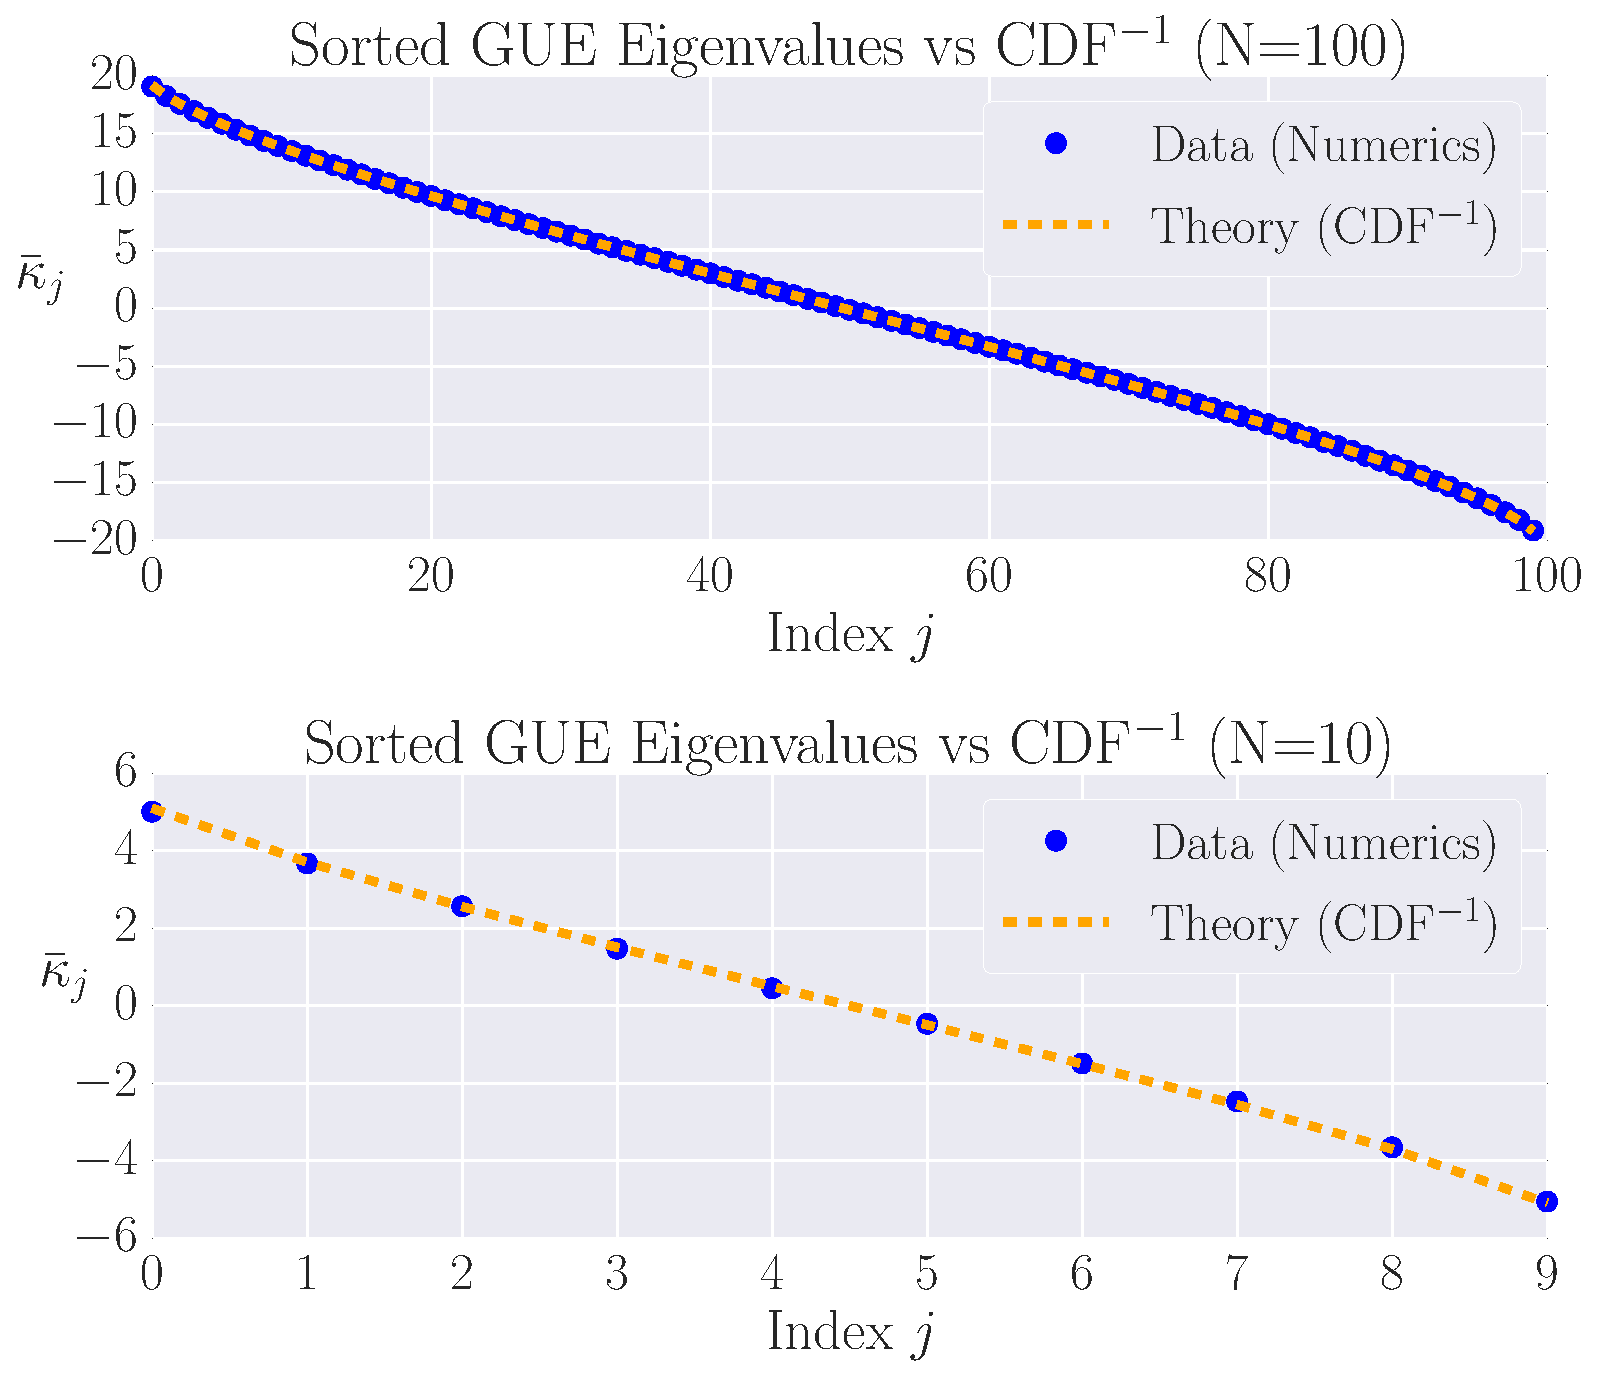
\includegraphics[width=\columnwidth]{Images/Figure_4.pdf}
\caption{Order statistics of the GUE($N$) eigenvalue distribution are very well approximated by the inverse CDF of the Wigner semicircle distribution.  In both figures, we compare the order statistics of a GUE($N$) distribution to the inverse CDF of the Wigner semicircle distribution. \textbf{Top}:  $N=100$.  \textbf{Bottom}:  $N=10$.
Agreement in both cases is essentially perfect.}
\label{fig:orderstatistics2}
\end{figure}

We make one further approximation, by assuming that $N\gg1$, so the distribution of the $\overline{\kappa}_j$ is effectively continuous and identical to $\mathrm{Pr}(\kappa)$. For the quantities that we compute, this is equivalent to replacing the empirical distribution function (which is a step function) by the CDF of the Wigner semicircle distribution.  So, whereas for any given sample the partial sum of all $\kappa_j > q$ jumps discontinuously when $q=\kappa_j$ for any $j$, in this approximation it changes smoothly.  This accurately models the \emph{average} behavior of partial sums.

\subsubsection{Deriving an Approximation for $q$}
The approximations of the previous section allow us to use the following ansatz for the eigenvalues of $\hat\rho$; namely, $\{p_j\} \cup \{\overline{\kappa}_j\}$, where the $p_j$ are $\mathcal{N}(\rho_{jj},\epsilon^2)$ random variables, and the $\overline{\kappa}_j$ are the (fixed, smoothed) order statistics of a Wigner semicircle distribution.  In turn, the defining equation for $q$ (Equation \eqref{eq:q_eqn}) is well approximated as
\begin{equation}
\sum_{j=1}^{r}(p_j - q)^{+} + \sum_{j=1}^{N}{(\overline{\kappa}_j-q)^+} \approx 1
\end{equation}
To solve this equation, we observe that the $\overline{\kappa}_j$ are symmetrically distributed around $
\kappa=0$, so half of them are negative.  Therefore, with high probability, $\Tr
\left[\mathrm{Trunc}(\hat\rho)\right]>1$, and so we will need to subtract $q\Id$ from $\hat\rho$ before truncating. (This is in distinction to the case where we have to \emph{add} $q$.)

We make another assumption; namely, that the eigenvalues of $\rho_{0}$ are large compared to the perturbations $\delta_{jj}$ and $q$. This implies $(p_{j} - q)^{+} = p_{j} - q$. Under this assumption, $q$ is the solution to
\begin{align}
\nonumber 1 &\approx \sum_{j=1}^{r}(p_j - q)^{+} + \sum_{j=1}^{N}{(\overline{\kappa}_j-q)^+}\\
\nonumber &\approx 1 - rq + \Delta + N\int_{\kappa=q}^{2\epsilon\sqrt{N}}{(\kappa-q)\mathrm{Pr}(\kappa)\mathrm{d}\kappa}\\
\label{eq:q_eqn2}\implies 0 &= - rq + \Delta + \frac{\epsilon}{12\pi}\left[
\begin{array}{l} (q^2+8N)\sqrt{-q^2+4N} \\
-12qN\left(\frac{\pi}{2}-\sin^{-1}\left(\frac{q}{2\sqrt{N}}\right)\right)
\end{array}\right],\nonumber\\
~
\end{align}
where $\Delta = \sum_{j=1}^{r}\delta_{jj}$ is a $\mathcal{N}(0,r\epsilon^2)$ random variable.  We choose to replace a discrete 
sum (line 1) with an integral (line 2). This approximation is valid when $N\gg1$, as we can accurately approximate a discrete collection of closely spaced real numbers by a smooth density or distribution over the real numbers that has approximately the same CDF.  It is also remarkably accurate in practice.
  
In yet another approximation, we replace $\Delta$ with its average value, which is zero.  We could obtain an even more accurate expression 
 by treating the fluctuations in $\Delta$ more carefully, but this crude approximation turns out to be quite accurate already.

To solve Equation \eqref{eq:q_eqn2}, it is necessary to further simplify the complicated expression resulting from the integral (line 3).  To do so, we 
assume  $\rho_0$ is relatively low-rank, so $r \ll N$.  In this case, the sum of the positive $\overline{\kappa}_j$ is large compared 
with $r$, almost all of them need to be subtracted away, and therefore $q$ is close to $2\epsilon\sqrt{N}$.  \footnote{This justifies the assumption that $\rho_{jj} + \delta_{jj} - q > 0$.} We therefore replace 
the complicated expression with its leading order Taylor expansion around $q=2\epsilon\sqrt{N}$, substitute into Equation \eqref{eq:q_eqn2}, and 
obtain the equation
\begin{equation}
\frac{rq}{\epsilon}  = \frac{4}{15\pi}N^{1/4}\left(2\sqrt{N}-\frac{q}{\epsilon}\right)^{5/2}.
\end{equation}
This equation is a quintic polynomial, so it has no closed-form solution.  However, its roots have a well-defined asymptotic ($N\to
\infty$) expansion that becomes accurate quite rapidly (e.g., for $N>4$):
\begin{equation}
\label{eq:truncation}
z \equiv q/\epsilon \approx 2\sqrt{N}-\frac{(240r\pi)^{2/5}}{4}N^{1/10}+\frac{(240r\pi)^{4/5}}{80}N^{-3/10}.
\end{equation}

\todo[inline]{Do we want a figure of how well this does?}

\subsubsection{Computing $\langle \lambda_{\mathrm{kite}}\rangle$}
Now that we know how much to subtract off in the truncation process, we can approximate $\expect{\lambda_{\mathrm{kite}}}$, originally given in Equation \eqref{eq:llrs_kite}:
\begin{align}
\nonumber \expect{\lambda_{\mathrm{kite}}} &\approx  \frac{1}{\epsilon^{2}}\left\langle\sum_{j=1}^{r}[\rho_{jj}- (p_j-q)^{+}]^2 + \sum_{j=1}^{N}\left[(\bar{\kappa}_j-q)^+\right]^2 \right\rangle\\
\nonumber &\approx \frac{1}{\epsilon^{2}} \left\langle\sum_{j=1}^{r}[-\delta_{jj} +  q ]^2 + \sum_{j=1}^{N}\left[(\bar{\kappa}_j-q)^+\right]^2 \right\rangle\\
\nonumber  &\approx r + rz^2 + \frac{N}{\epsilon^{2}}\int_{\kappa=q}^{2\epsilon\sqrt{N}}{ \mathrm{Pr}(\kappa)(\kappa-q)^2 d\kappa} \\
\nonumber &=r + rz^{2} + \frac{N(N+z^{2})}{\pi}\left(\frac{\pi}{2} - \sin^{-1}\left(\frac{z}{2\sqrt{N}}\right)\right) \\
& - \frac{z(z^{2}+26N)}{24\pi}\sqrt{4N-z^{2}}
\end{align}

\section{Result for $\langle \lambda \rangle$, Comparison to Numerical Experiments}
The total expected value, $\expect{\lambda} = \expect{\lambda_{\mathrm{L}}} + \expect{\lambda_{\mathrm{kite}}}$, is thus
\begin{align}
\label{eq:ourLLRS}
\nonumber \langle \lambda(\rho_{0}, \M_{d}) \rangle &\approx 2rd - r^{2}+rz^{2}\\
\nonumber & + \frac{N(N+z^{2})}{\pi}\left(\frac{\pi}{2} - \sin^{-1}\left(\frac{z}{2\sqrt{N}}\right)\right) \\
& - \frac{z(z^{2}+26N)}{24\pi}\sqrt{4N-z^{2}}
\end{align}
where $z$ is given in Equation \eqref{eq:truncation}, $N=d-r$, and $r = \mathrm{Rank}(\rho_{0})$.

Equation \eqref{eq:ourLLRS} is our main result.  To test its validity, we compare it to numerical simulations for $d=2,\ldots,30$ and $r=1,\ldots,10$, in Figure \ref{fig:modelcomp-iso}.  The prediction of the Wilks Theorem is wildly incorrect for $r\ll d$. In contrast, Equation \eqref{eq:ourLLRS} is almost perfectly accurate when $r \ll d$, but it does begin to break down (albeit fairly gracefully) as $r$ becomes comparable to $d$.  We conclude that our analysis (and Equation \eqref{eq:ourLLRS}) correctly models tomography \emph{if} the Fisher information is isotropic ($\Fi \propto \Id$).

\begin{figure}[h]
 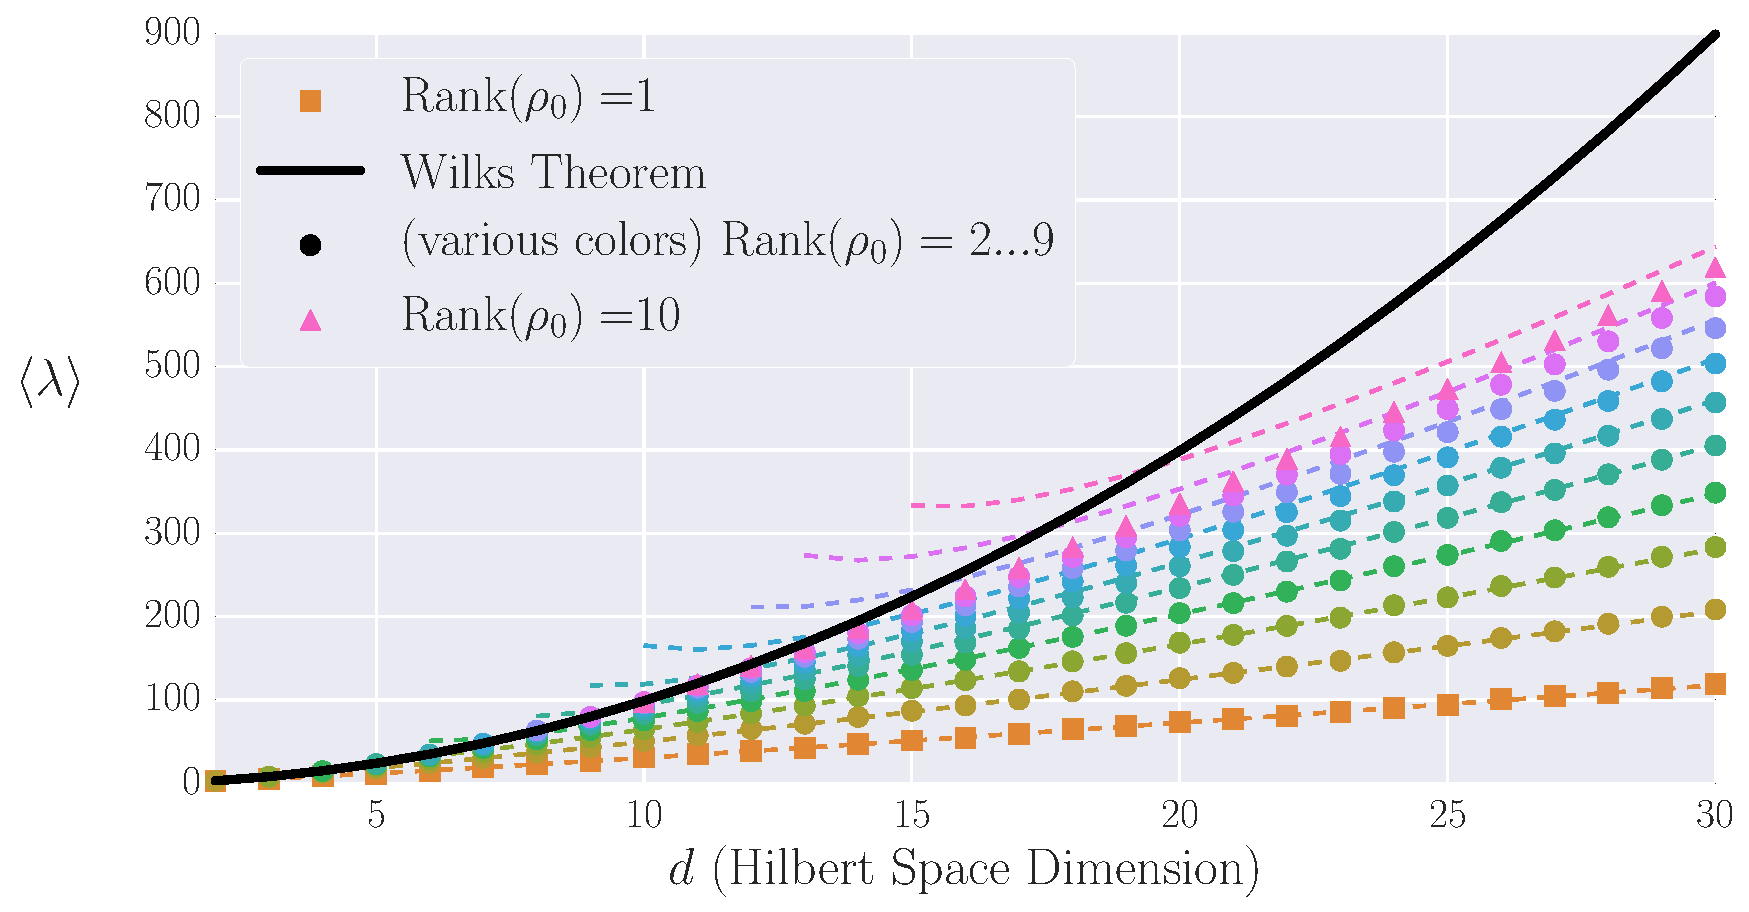
\includegraphics[width=\columnwidth]{Images/Figure_5.pdf}
 \caption{Numerical results for $\expect{\lambda}$ compared to the prediction of the Wilks Theorem (solid line) and our replacement theory as given in Equation \eqref{eq:ourLLRS}, (dashed lines).  Our formula depends on the rank $r$ of $\rho_0$ (unlike the Wilks prediction), and is nearly perfect for $r\ll d$.  It becomes less accurate as $r$ approaches $d/2$, and is invalid when $r\approx d$.}
 \label{fig:modelcomp-iso}
\end{figure}

\section{Comparison to Heterodyne Tomography}
In practice, the Fisher information is rarely isotropic.  So we tested our idealized result by applying it to a realistic, challenging, and experimentally relevant problem: quantum heterodyne (equivalent to double homodyne) state tomography \cite{Lvovsky2001a, Bertrand1987, Leonhardt1995, Lvovsky2009} of a single optical mode.  (See Figure \ref{fig:fish_condition} for a plot of the \emph{condition number} -- the ratio of the largest to smallest eigenvalue -- of the estimated Fisher information. It is clear that, for such a tomographic setup, $\mathcal{I} \not \propto \Id$.) States of this continuous-variable system are described by density operators on the infinite-dimensional Hilbert space $L^2(\reals)$.  Fitting these infinitely many parameters to finitely much data demands simpler models.

We consider a family of nested models motivated by a low-energy (few-photon) ansatz, and choose   
the Hilbert space $\mathcal{H}_d$ to be that spanned by the photon number states $\{\ket{0},\ldots ,\ket{d-1}\}$.
Heterodyne tomography reconstructs $\rho_{0}$ using data from repeated measurements of the 
coherent-state POVM, $\{|\alpha\rangle\langle \alpha| /\pi, ~\alpha=x+ip\in \mathbb{C}\}$, which corresponds to sampling directly from the 
state's Husimi $Q$-function \cite{Husimi1940}.

\begin{figure}[h]
  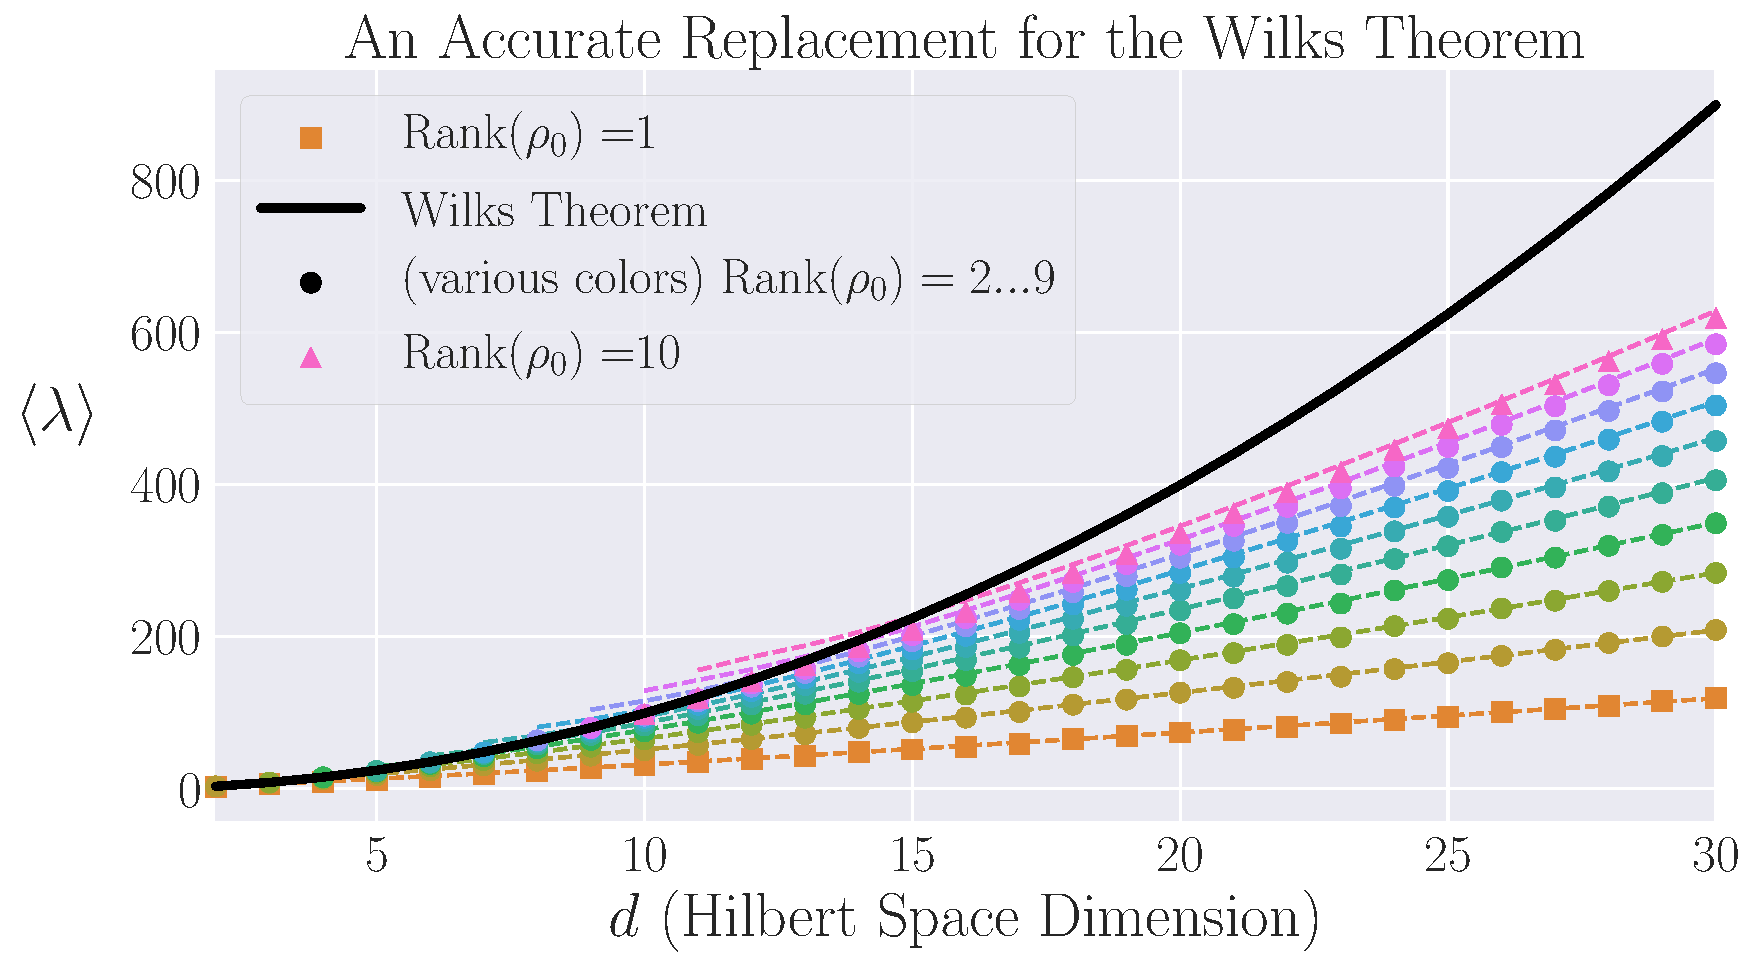
\includegraphics[width=\columnwidth]{Images/Figure_6.pdf}
 \caption{The condition number $\kappa$ -- the ratio of the largest to smallest eigenvalue -- of the estimated heterodyne Fisher information grows with model dimension, indicating an increase in anisotropy. (Estimates are the average over 100 Hessians of the loglikelihood function.) The dashed lines indicate different states $\rho_{0}$, and the solid line is $\kappa = 1$ (i.e., $\mathcal{I} \propto \Id$.).}
\label{fig:fish_condition}
\end{figure}

We examined the behavior of $\lambda$ for 13 distinct states $\rho_{0}$, both pure and mixed, supported on $\mathcal{H}_{2}, \mathcal{H}_{3}, \mathcal{H}
_{4}$, and $\mathcal{H}_{5}$.  We used rejection sampling to simulate 100 heterodyne datasets with up to $N_{\mathrm{samples}}=10^5$, and found MLEs over each of the 9 models $\M_2, \ldots, M_{10}$ using numerical optimization \footnote{The model $\M_{1}$ is trivial, as $\M_{1} = \{|0\rangle \langle 0|\}$. This model will almost always be wrong, in general.}.  For each $\rho_{0}$ and each $d$, we averaged $\lambda(\rho_{0}, \M_{d})$ over all 100 datasets to obtain an empirical average loglikelihood ratio $\bar{\lambda}$ for each $(\rho_0,d)$ pair.

\begin{figure}[h]
 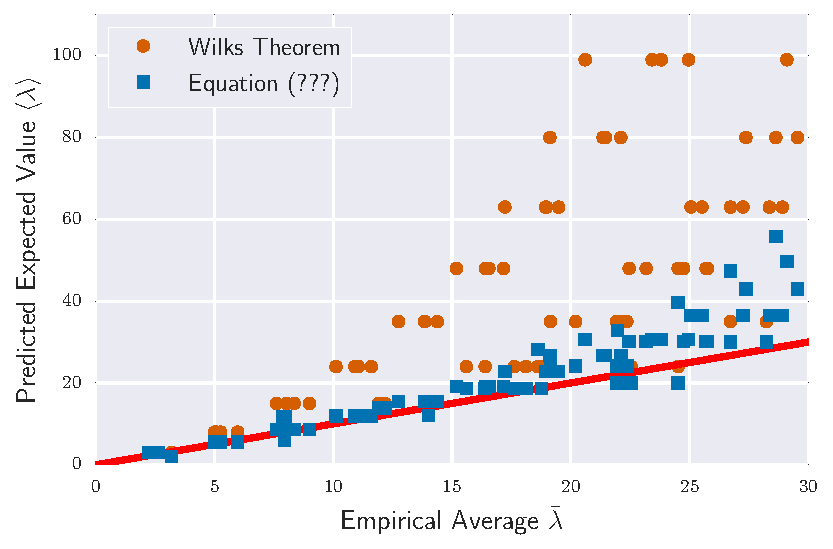
\includegraphics[width=\columnwidth]{Images/Figure_7.pdf}
 \caption{The Wilks Theorem (orange dots) dramatically over-estimates $\langle\lambda(\rho_{0}, \M_{d})\rangle$ in optical heterodyne tomography. Our formula, Equation \ref{eq:ourLLRS} (blue squares), is far more accurate. Residual discrepancies occur in large part because $N_{\mathrm{samples}}$ is not yet ``asymptotically large''. The solid red line corresponds to perfect correlation between theory ($\expect{\lambda}$) and practice ($\bar\lambda$).}
 \label{fig:modelcomp}
\end{figure}

Results of this test are shown in Figure \ref{fig:modelcomp}, where we plot the predictions for $\langle \lambda \rangle$ given by the Wilks Theorem and Equation \eqref{eq:ourLLRS}, against the empirical average $\bar\lambda$, for a variety of $\rho_{0}$ and $d$. Our formula correlates very well with the empirical average, while the Wilks Theorem (unsurprisingly) overestimates $\lambda$ dramatically for low-rank states.  Whereas a model selection procedure based on Wilks Theorem would tend to falsely reject larger Hilbert spaces (by setting the threshold for acceptance too high), our formula provides a reliable null theory.

Interestingly, as $d$ grows, Equation \eqref{eq:ourLLRS} also begins to overpredict. As Figure \ref{fig:totalcontrib} indicates, a more accurate description is that the numerical experiments are \emph{underachieving}, because $\bar\lambda$ is still growing with $N_{\mathrm{samples}}$.  Both the Wilks Theorem and our analysis are derived in an asymptotic limit $N \rightarrow \infty$; for finite but large $N$, both may be invalid.  Figure \ref{fig:totalcontrib} shows that, even at $N\sim 10^{5}$, the behavior of $\bar{\lambda}$ has failed to become asymptotic. This is surprising, and suggests heterodyne tomography is a particularly exceptional and challenging case to model statistically. 

\begin{figure}[h]
  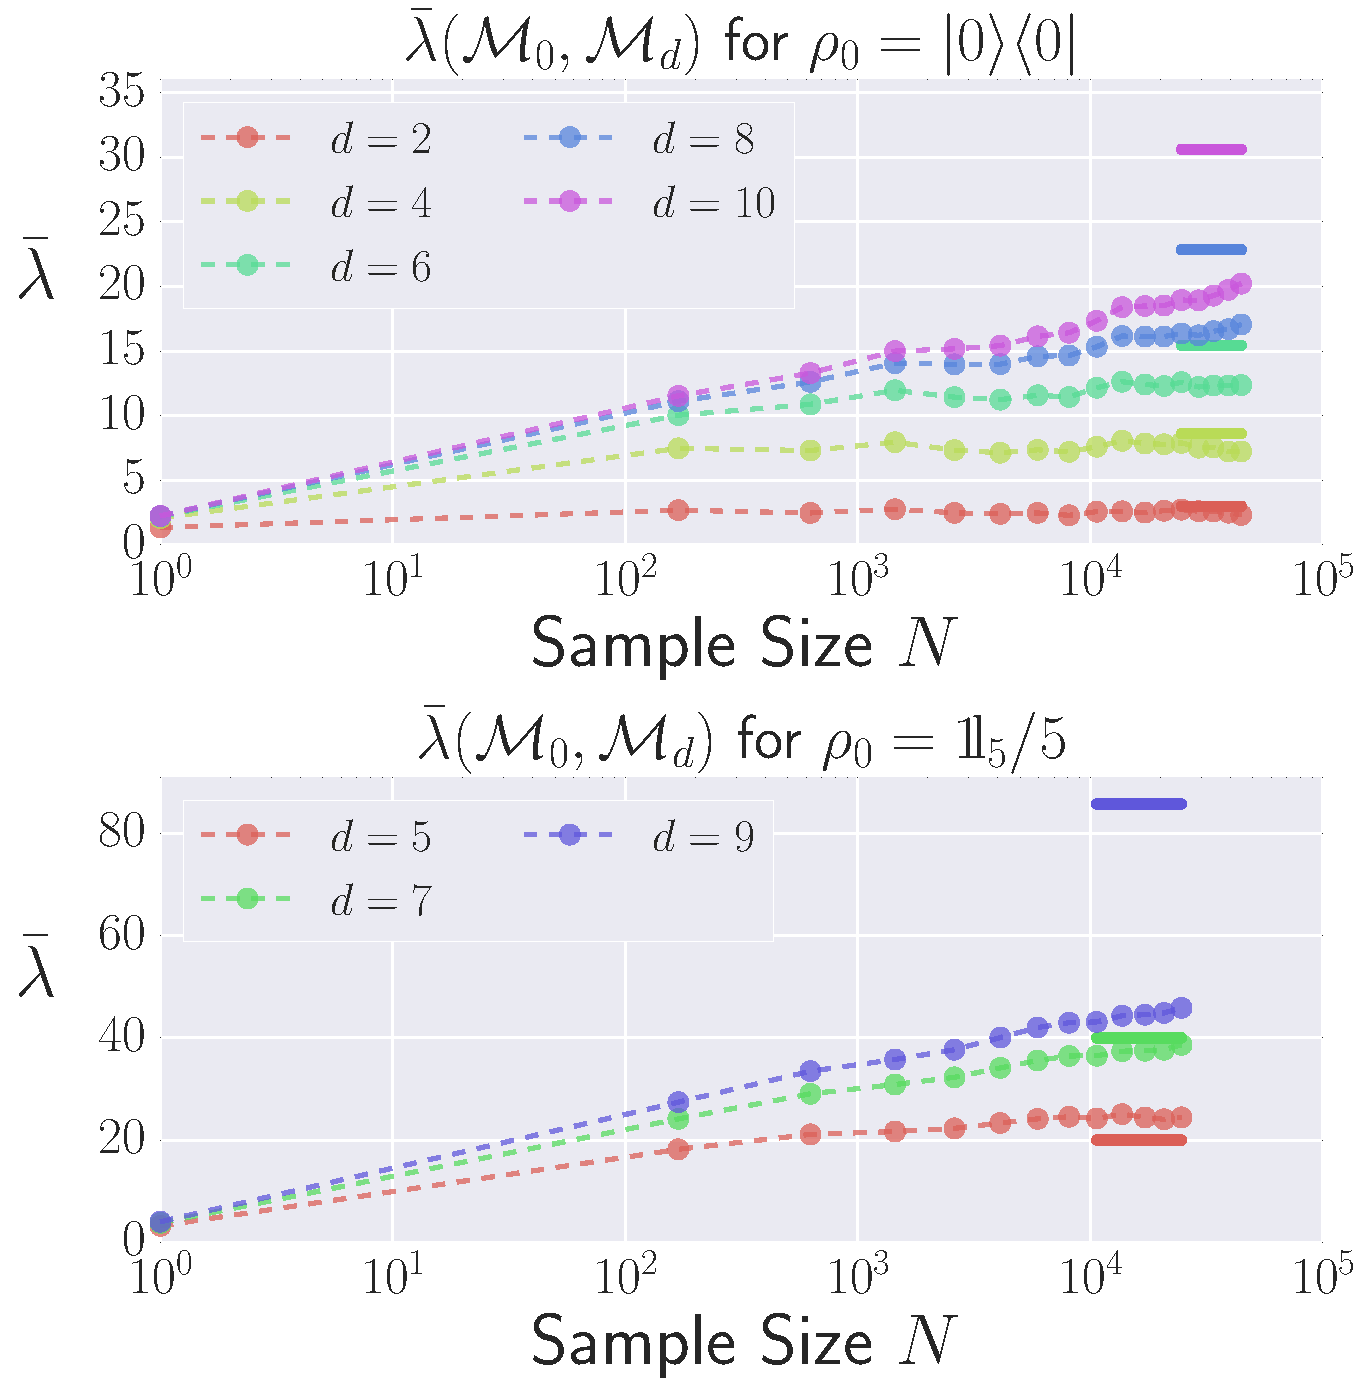
\includegraphics[width=\columnwidth]{Images/Figure_8.pdf}
 \caption{The empirical average $\bar{\lambda}$  may have achieved its asymptotic value, or is still 
growing, depending on the true state $\rho_{0}$ and the model dimension $d$. Solid lines indicate the value of our formula
for the asymptotic expected value, given in Equation \eqref{eq:ourLLRS}.}
\label{fig:totalcontrib}
\end{figure}


However, our model \emph{does} get some of the qualitative features correct. In Figure \ref{fig:model_comparison}, we look at $\langle \lambda_{jk}\rangle$, where we assume an isotropic Fisher information, and when we simulate heterodyne tomography. While the numbers given for $\langle \lambda_{jk} \rangle$ do not agree exactly, they still break down into two groups, the ``L" and the ``kite". (See Figure \ref{fig:individcontrib} for an analysis of the exact differences in the values.)
 
 
\begin{figure}[h]
  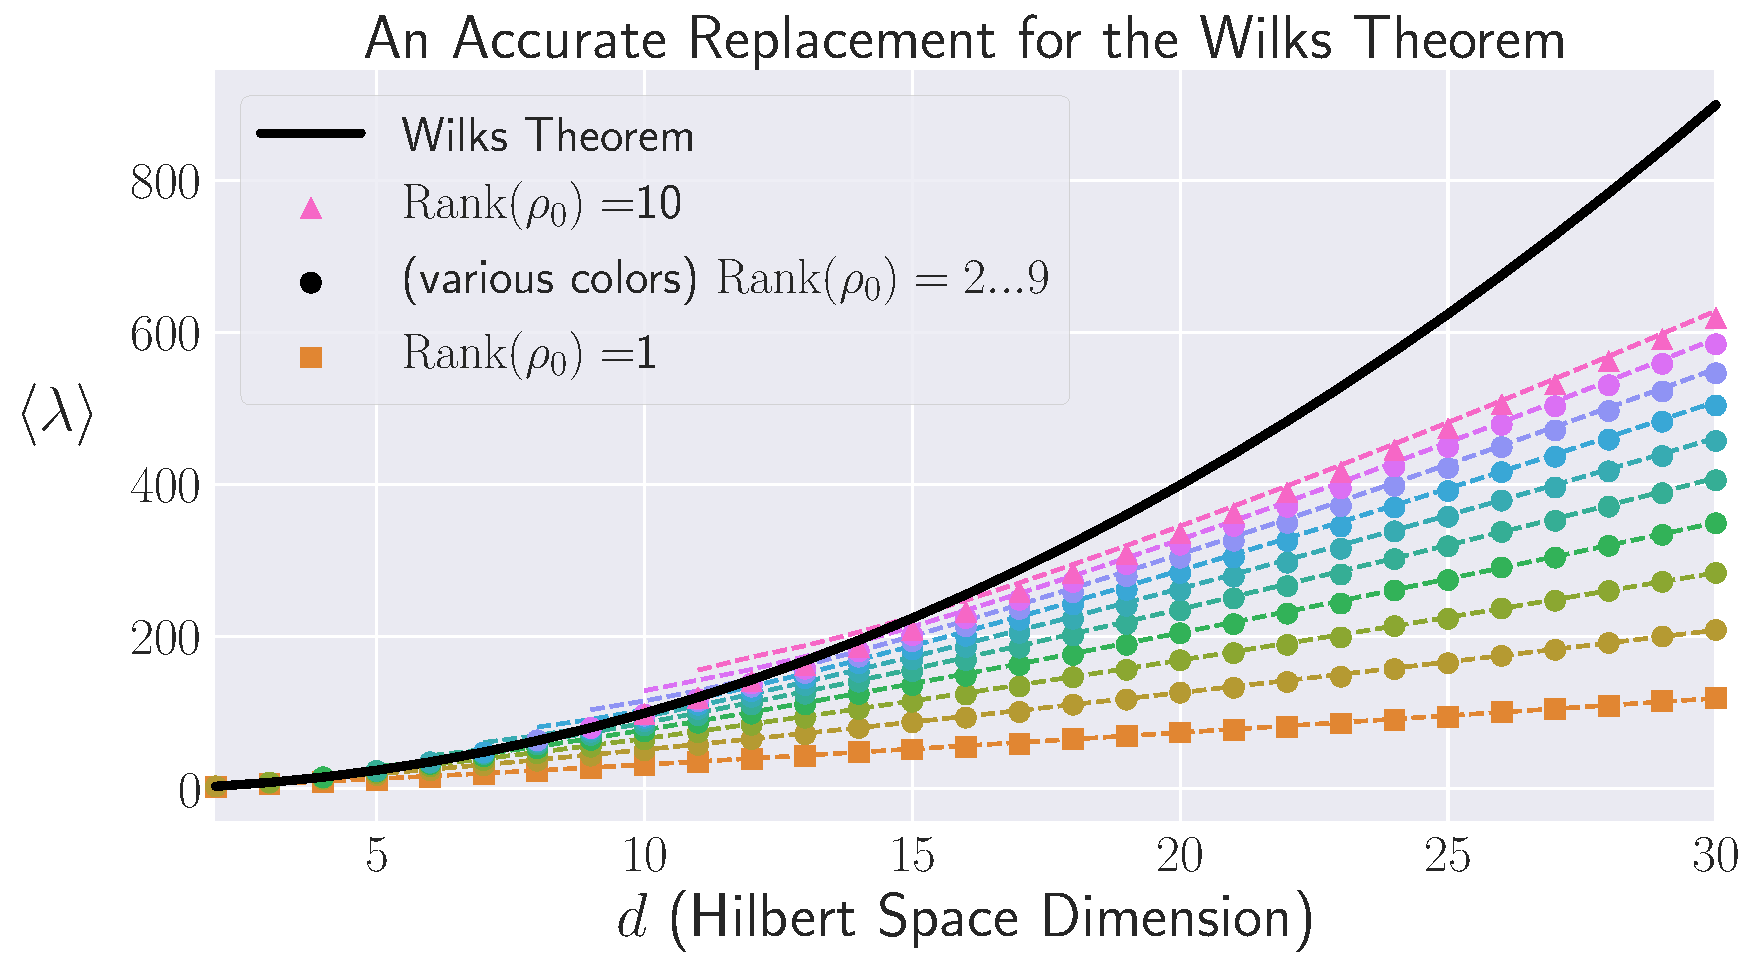
\includegraphics[width=\columnwidth]{Images/Figure_9.pdf}
 \caption{The values of $\langle \lambda_{jk} \rangle$ assuming an isotropic Fisher information (left), and for heterodyne tomography (right). \textbf{Top}: $\rho_{0} = |0\rangle\langle 0|$. \textbf{Bottom}: $\rho_{0} = \mathcal{I}_{2}/2$. \textbf{Discussion}: Qualitatively, the behavior is the same, though there are quantitative differences, particularly within the kite.}
\label{fig:model_comparison}
\end{figure}

\begin{figure}[h]
  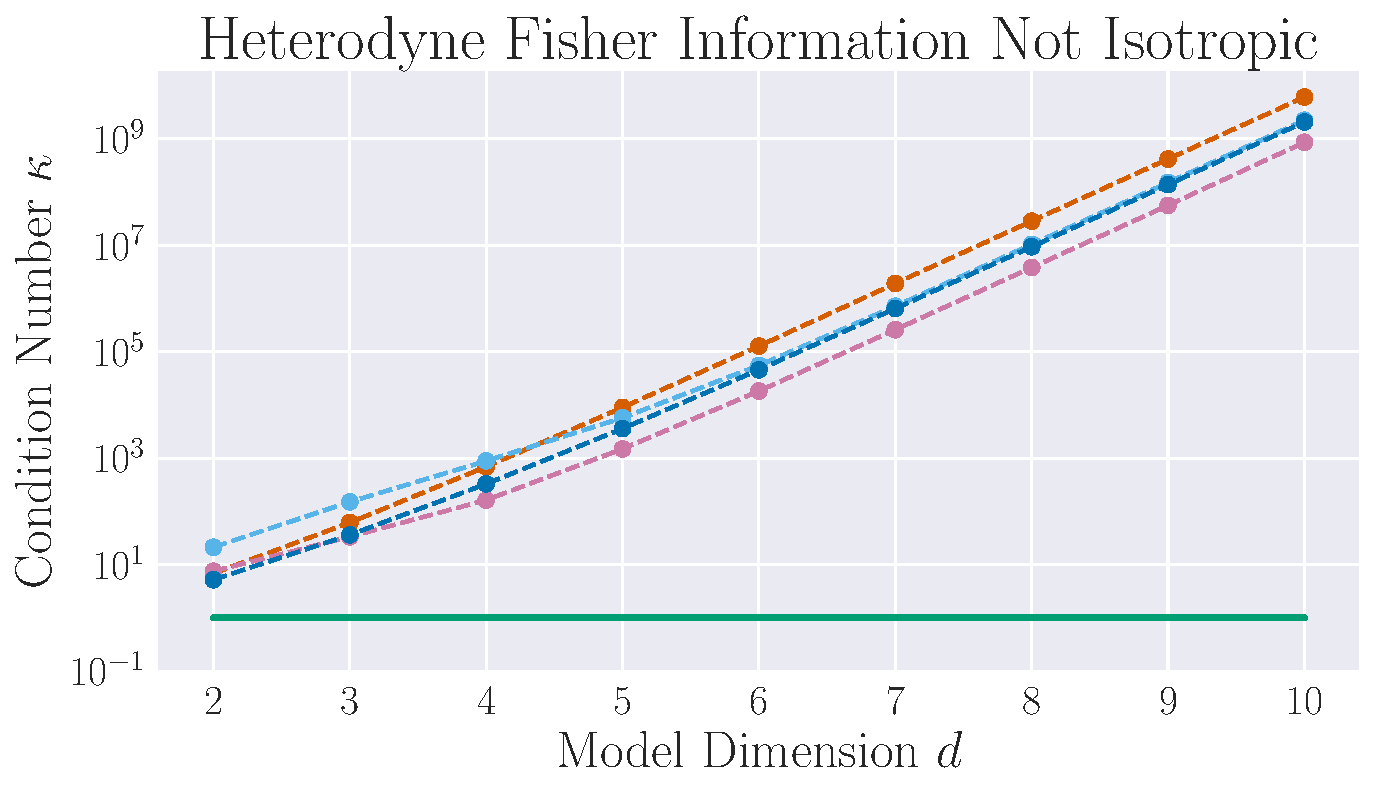
\includegraphics[width=\columnwidth]{Images/Figure_10.pdf}
 \caption{Examining how our predicted values for $\langle \lambda_{jk} \rangle$ disagree with simulated heterodyne experiments. We take $\rho_{0} = |0\rangle\langle 0|$ and $d=8$. \textbf{Top Left}: The values of  $\langle \lambda_{0k}\rangle$ in the ``L" as a function of sample size $N$.  \textbf{Top Right}:  Even at the largest $N$ studied, $\langle \lambda_{0k}\rangle$ is nontrivially less than 1, especially for the higher number states. \textbf{Bottom Left}: The total from the ``kite" versus $N$. It is clear the total is still growing. \textbf{Bottom Right}: The individual ``kite" elements $\langle \lambda_{jk}\rangle$ at the largest $N$ studied;  most are small compared to values they would have in the isotropic case.}
\label{fig:individcontrib}
\end{figure}



\section{Conclusions and Discussion}
The Wilks Theorem is not generally reliable in quantum state tomography, but our Equation \eqref{eq:ourLLRS} provides a much more broadly applicable replacement that can be used in model selection methods.  This includes protocols like the AIC and BIC \cite{Akaike1974, Schwarz1978, Kass1995, Burnham2004} that do not explicitly use the Wilks Theorem, but rely on the same assumptions (asymptotic normality, etc).  Null theories of loglikelihood ratios have many other applications, including hypothesis testing \cite{Blume-Kohout2010,Moroder2013} and confidence regions \cite{Glancy2012a}, and our result is directly applicable to them.  Refs. \cite{Moroder2013,Glancy2012a} both point out explicitly that their methods are unreliable near boundaries and therefore cannot be applied to rank-deficient states; our result fixes this outstanding problem.  However, our numerical experiments with heterodyne tomography show unexpected behavior, indicating that quantum tomography can still surprise, and may violate \emph{all} asymptotic statistics results.  In such cases, bootstrapping \cite{Efron1979, Higgins2004} may be the only reliable way to construct null theories for $\lambda$.  Finally, the \emph{methods} presented here have application beyond the analysis of loglikelihoods.  They shed light on the behavior of $\rhoMLE$ for rank-deficient states, and can be used to predict other derived properties such as the average rank of the estimate, which is independently interesting for (e.g.) quantum compressed sensing \cite{Flammia2012a, Steffens2016, Kalev2015, Kalev2015a}.

\section{Acknowledgements:} The authors are grateful for those who provide support for the following software packages: iPython/Jupyter \cite{Perez}, matplotlib
\cite{Hunter2007}, mpi4py \cite{Dalcin2011},  NumPy \cite{VanDerWalt2011}, pandas \cite{mckinney2010}, Python 2.7 
\cite{vanRossum}, seaborn \cite{Waskom2016}, and SciPy \cite{Oliphant2007a}. TLS thanks Jonathan A Gross for helpful 
discussions on software design, coding, and statistics, John King Gamble for useful insights on parallelized 
computation and feedback on earlier drafts of this paper, and Daniel Seuss for proofreading edits.

Sandia National Laboratories is a multi-mission laboratory managed and operated by Sandia Corporation, a wholly owned 
subsidiary of Lockheed Martin Corporation, for the U.S. Department of Energy's National Nuclear Security Administration 
under contract DE-AC04-94AL85000.

\bibliographystyle{apsrev4-1}
\bibliography{wilkspaper}
\end{document}
